\documentclass[12pt,a4paper,utf8]{ctexart}
\usepackage{ctex,amsmath,amssymb,subfig,cite,graphicx,diagbox,fontspec,fancyhdr,geometry}
\usepackage[ntheorem]{empheq}
\usepackage{enumitem,fullpage,cleveref,cellspace,listings,color,framed}
\definecolor{gray}{rgb}{0.5,0.5,0.5}
\definecolor{dkgreen}{rgb}{.068,.578,.068}
\definecolor{dkpurple}{rgb}{.320,.064,.680}

%set Fortran styles
\lstset{
    frameround=tftf,
    language=Fortran,
    keywords={SELECT,PROGRAM,PRINT,STOP,END,WRITE,INTEGER,REAL,COMPLEX,CHARACTER,LOGICAL,READ,FORMAT,IMPLICIT,PARAMETER,DATA,EQUIVALENCE,TYPE,PAUSE,CONTINUE,CYCLE,EXIT,IF,SELECT,DO,ALLOCATE,DEALLOCATE,WHERE,FORALL,SUBROUTIHNE,CALL,RETURN,FUNCTION,COMMON,BLOCK DATA,SAVE,INTERFACE,CONTAIN,MODULE,USE,PUBLIC,PRIVATE,ENTRY,OPEN,INQUIRE,CLOSE,NAMELIST,POINTER,NULLFY,REWIND,BACKSPACE,ENDFILE
    },
    basicstyle=\small\ttfamily,
    numbers=left,
    numberstyle=\small,
    keywordstyle=\color{blue}\bfseries,
    commentstyle=\color{dkgreen},
    stringstyle=\color{dkpurple},
    backgroundcolor=\color{white},
    tabsize=2,
    showspaces=false,
    showstringspaces=false,
    breaklines=true,
    frame=trBL,
}
\CTEXsetup[format+={\raggedright}]{section}
\setlength{\parindent}{2em}
\geometry{
    textwidth=138mm,
    textheight=215mm,
    left=27mm,
    right=27mm,
    top=25.4mm,
    bottom=25.4mm,
    headheight=2.17cm,
    headsep=4mm,
    footskip=12mm,
    heightrounded,
}
\pagestyle{fancy}
\lhead{\textsl{2021秋-计算物理A}}
\chead{}
\rhead{\textsl{PB19020634-于浩然}}
\lfoot{}
\cfoot{\thepage}
\rfoot{}

\begin{document}
\begin{center}
    {\LARGE\textbf{计算物理作业九}}\\
    \textrm{于浩然}~~~~~~\textrm{PB19020634}~~~~~~\textrm{2021.10.20}
\end{center}

\section{作业题目}

考虑泊松分布、指数分布,并再自设若干个随机分布(它们有相同或不同的 $\mu$和$\sigma
^2$),通过Monte Carlo模拟,验证中心极限定理成立($N=2,5,10$).

\section{算法简介}

\subsection{中心极限定理}

概率论中大数法则和中心极限定理是Monte
Carlo方法应用于统计计算的基础.大数法则说,若随机量序列${f_i}$有期望值$\mu$,则
\begin{equation}
    \lim_{N\rightarrow \infty} \frac{1}{N} \sum_{i=1}^{N}f_i \rightarrow \mu
\end{equation}

而中心极限定理指出了当$N$有限时,平均值的误差分布.即
\begin{equation}
    P \left\{ \bigg|\frac{\langle f \rangle - \mu}{\sigma_f / \sqrt{N}} \bigg|  <
    \beta\right\} \rightarrow \Phi(\beta)
\end{equation}

其中$\Phi(\beta)$是Gauss正态分布.因此
\begin{equation}
    \sigma_s = \left| \langle f \rangle - \mu \right| \propto
    \frac{\sigma_f}{\sqrt{N}} = \frac{1}{\sqrt{N}} 
    \sqrt{\langle f^2 \rangle - \langle f \rangle ^2}
\end{equation}

上式中$\sigma_f$是函数$f(x)$的标准差,$\sigma_s$是积分值的标准差.

若要验证此定理,可以对满足任一分布的随机变量$x$进行$N$次抽样,计算统计量
$\frac{\langle x \rangle - \mu}{\sigma / \sqrt{N}}$,重复上述过程$n$次取平均,
可得到对应分布抽样$N$次所得统计量的近似概率分布.将该概率分布与标准正态分布比较,
若随着$n$的增大两者越来越接近,则可认为中心极限定理成立.

\subsection{标准正态分布}

期望为0,方差为1的正态分布称为 \textbf{标准正态分布}. 其概率密度分布函数为
\begin{equation}
    f(x) = \frac{1}{\sqrt{2\pi}}e^{-x^2/2}
\end{equation}

其累积函数为
\begin{equation}
    \Phi(x) = \int _{-\infty} ^{x} f(t) \textrm{d}t 	
\end{equation}
\subsection{分布一:泊松分布}

若$X$服从参数为$\lambda$的泊松分布,记为$X \sim P(\lambda)$.
其概率密度分布函数(离散分布)为
\begin{equation}
    P(x = k) = \frac{\lambda^k}{k!}e^{-\lambda}, k = 0, 1,\cdots
\end{equation}

其期望值和标准差值可由参数$\lambda$确定:
\begin{equation}
    \mu = \sigma^2 = \lambda
\end{equation}

不妨取参数$\lambda = 2$,并构造如下统计量:
\begin{equation}
    g = \frac{ \bar{X} - \mu}{\sigma/\sqrt{N}} 
    = \sqrt{ \frac{N}{2}}(\bar{X} - 2)
\end{equation}

此分布中随机变量$X$取值为可数无穷多个,但实际上当$X$较大时取值概率已相当小
,故我们忽略后面的部分进行抽样.

$\lambda=2$时$P(X=k) =
\frac{2^k}{k!}e^{-2}$,这时$P(X=7)=0.0034$,$P(X=8)=0.00086$
,$P(X=9)=0.00019$,我们可以认为当$k > 8$时,$P(X=k) \approx 0$. 抽样时,
只需对$X=k(k=1,2,\cdots,8)$进行抽样.但由于后面仍有无穷多项,仍需重新归一化.
\subsection{分布二:指数分布}

若$X$服从参数为$\lambda$的指数分布,记为$X \sim E(\lambda)$.
其概率密度分布函数(连续分布)为
\begin{equation}
    f(x) = \lambda e^{-\lambda x}, \quad x \geq 0
\end{equation}

同样,我们可确定期望与方差:
\begin{equation}
    \langle x \rangle = \frac{1}{\lambda},\quad \sigma^2 = \frac{1}{\lambda^2}
\end{equation}

取参数$\lambda=1$,可构造统计量:
\begin{equation}
    g = \frac{ \bar{x} - 1/\lambda}{1/\lambda \sqrt{N}} 
    = \sqrt{N}(\bar{x} - 1)
\end{equation}

与Poisson分布同理,数值计算模拟时必须选取一段有限区间.
绘制参数$\lambda=1$的指数分布的概率密度函数图像展示如下:

\begin{figure}[t]
    \centering
    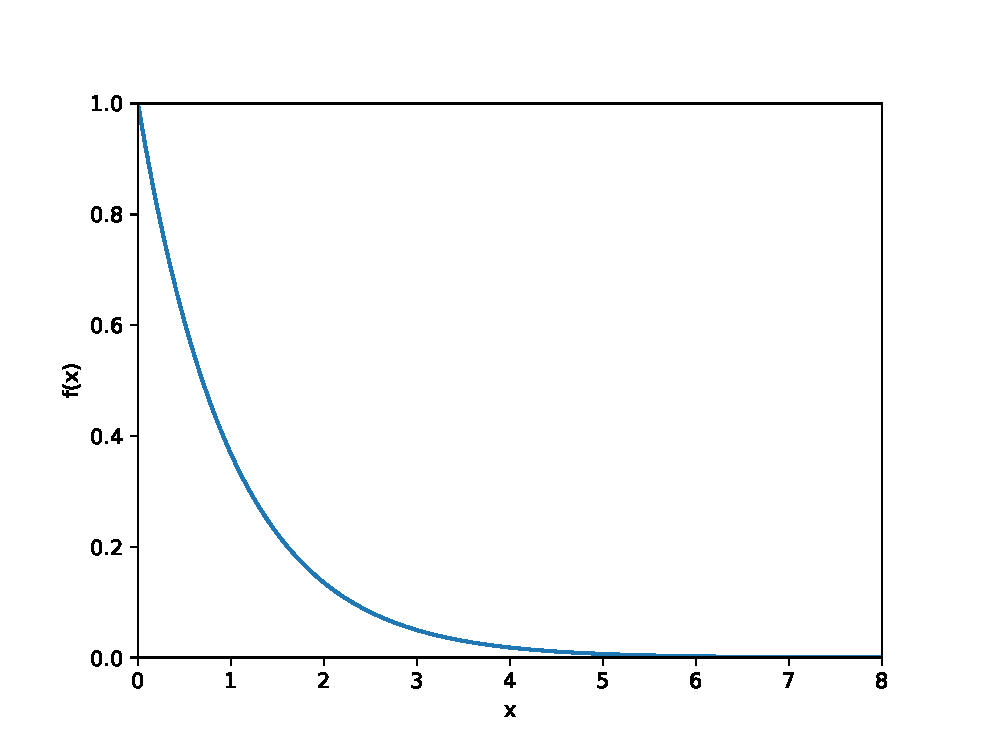
\includegraphics[width=0.8\textwidth]{fig_1.eps}
    \caption{$\lambda=1$的指数分布概率密度函数$f(x)$}
\end{figure}

显见,可忽略$x > 6$的部分,抽样时仅对$0 \leq x \leq 6$进行即可.

考虑直接抽样,对(9)式积分求出指数分布的累积函数:
\begin{equation}
    \xi(x) = \int _{0} ^{x} e^{-t} \textrm{d}t	 = 1 - e^{-x}
\end{equation}

求反函数:
\begin{equation}
    x = -\ln (1 - \xi) = -\ln(\xi)
\end{equation}

其中$\xi$为均匀分布随机变量,$\xi$与$1-\xi$等价.在编写抽样程序时
,可由上式从均匀随机数$\xi$抽出服从指数分布的$x$.
\newpage
\subsection{分布三:自设离散分布}

设分布函数为

\begin{equation}
    P(x = k) = 1/5,\quad k = 1, 2, 3, 4, 5
\end{equation}

容易计算其期望和方差:
\begin{equation}
    \langle X \rangle = 3,\quad \sigma^2 = 
    \langle X^2 \rangle - \langle X \rangle ^2 = 2
\end{equation}

可构造统计量:
\begin{equation}
    g = \frac{ \bar{X} - 3}{\sqrt{2/N}}
\end{equation}
\subsection{分布四:自设连续分布}

设分布函数为
\begin{equation}
    f(x) = x,\quad 0 \leq x \leq 1
\end{equation}

易得期望和方差
\begin{equation}
    \langle x \rangle = \frac{1}{3},\quad \sigma^2 = 
    \langle x^2 \rangle - \langle x \rangle ^2 = \frac{5}{36}
\end{equation}

可构造统计量:
\begin{equation}
    \frac{\bar{x} - 1/3}{\sqrt{5/36}/\sqrt{N}}=
    2 \sqrt{ \frac{N}{5}} (3\bar{x}-1)
\end{equation}

同样考虑进行直接抽样,累积函数为

\begin{equation}
    \xi(x) = \int _{0} ^{x} f(t) \textrm{d}t	= \frac{x^2}{2}
\end{equation}
求反函数:
\begin{equation}
    x = \sqrt{2\xi}
\end{equation}

于是可由上式抽样.

\section{编程实现}

用FORTRAN90进行编程,分别将离散抽样的两个子程序和连续(直接抽样)的两个子程序装在两个
模块中,便于管理与维护. 源代码较长,展示于报告最后.

\section{计算结果}

适当选取分割区间,用各组数据绘制直方图.
\subsection{泊松分布抽样结果}

\begin{figure}[htb]
    \centering
    \subfloat[$n=10^2$]{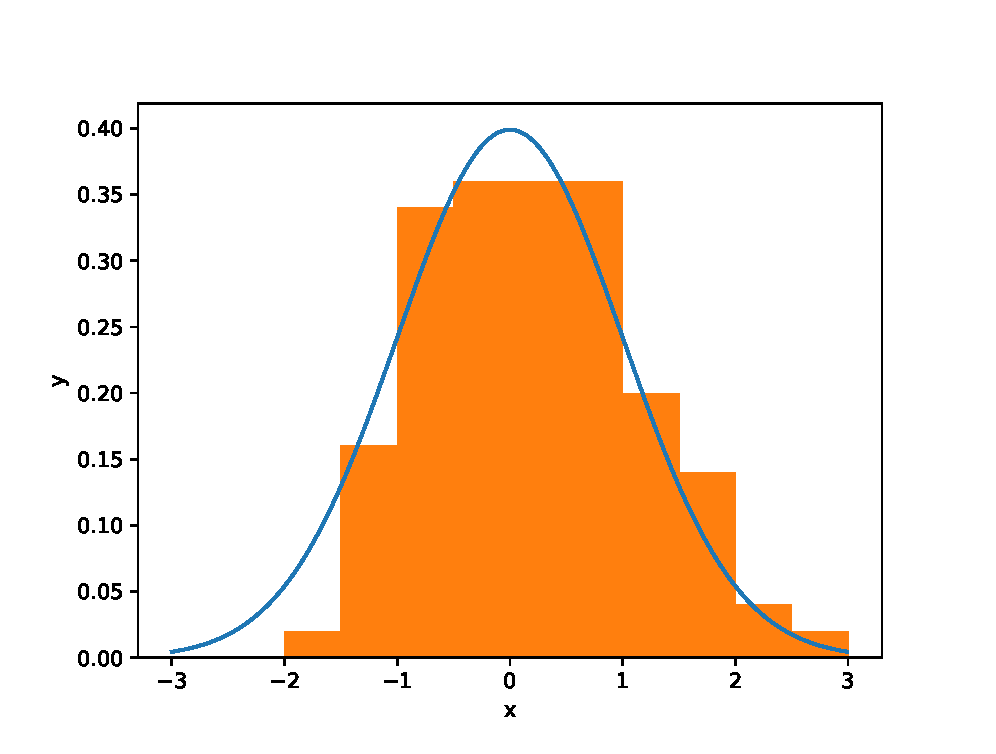
\includegraphics[width=0.33\textwidth]{poi_2_2.eps}}
    \hfill
    \subfloat[$n=10^4$]{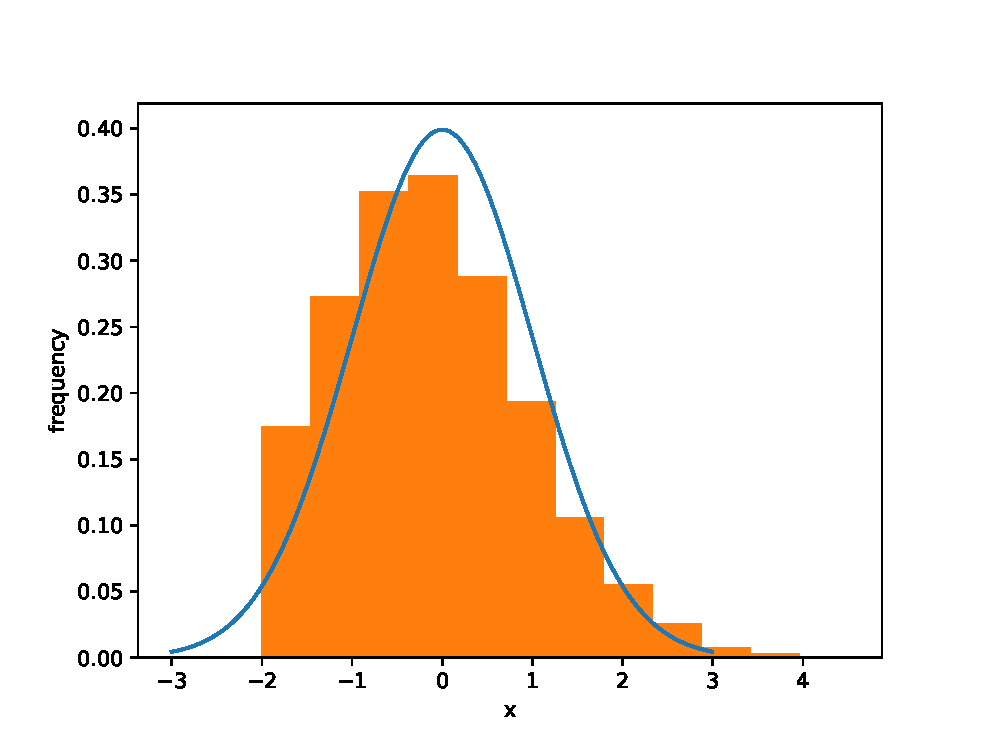
\includegraphics[width=0.33\textwidth]{poi_2_4.eps}}
    \hfill
    \subfloat[$n=10^6$]{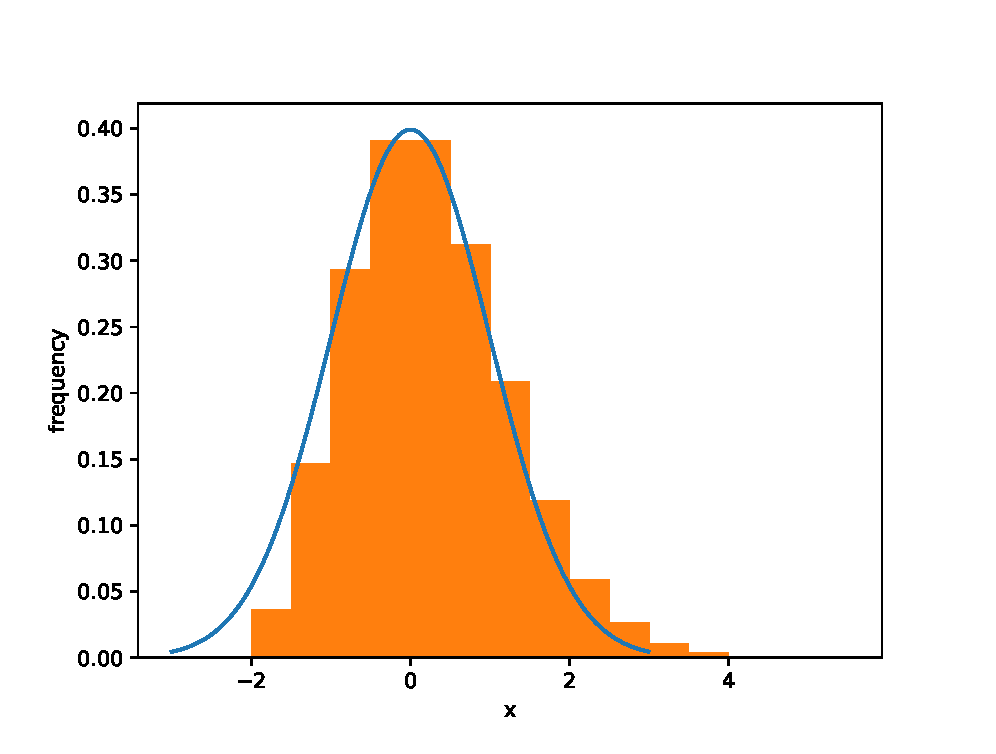
\includegraphics[width=0.33\textwidth]{poi_2_6.eps}}
    \hfill
    \caption{泊松分布抽样结果(N=2)}
\end{figure}
\begin{figure}[htb]
    \centering
    \subfloat[$n=10^2$]{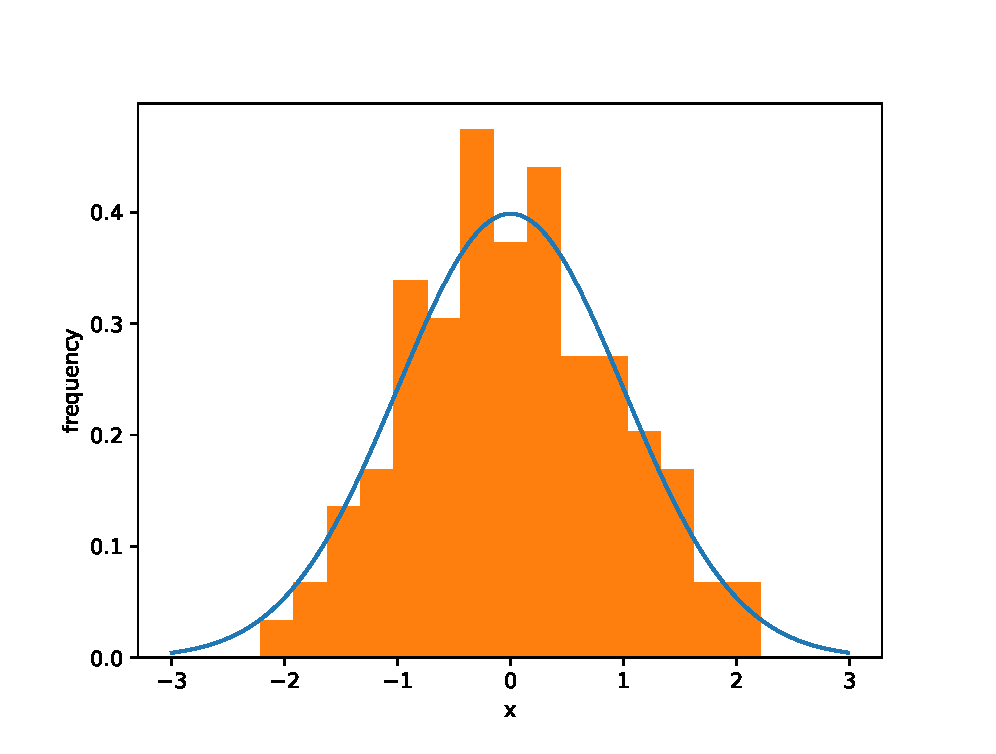
\includegraphics[width=0.33\textwidth]{poi_5_2.eps}}
    \hfill
    \subfloat[$n=10^4$]{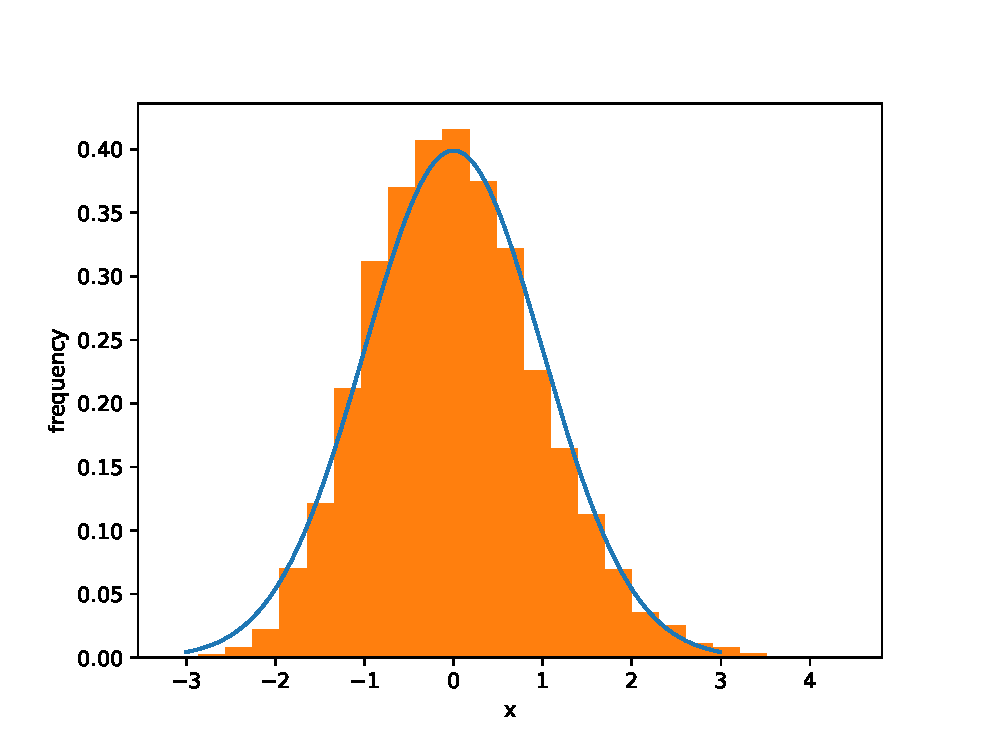
\includegraphics[width=0.33\textwidth]{poi_5_4.eps}}
    \hfill
    \subfloat[$n=10^6$]{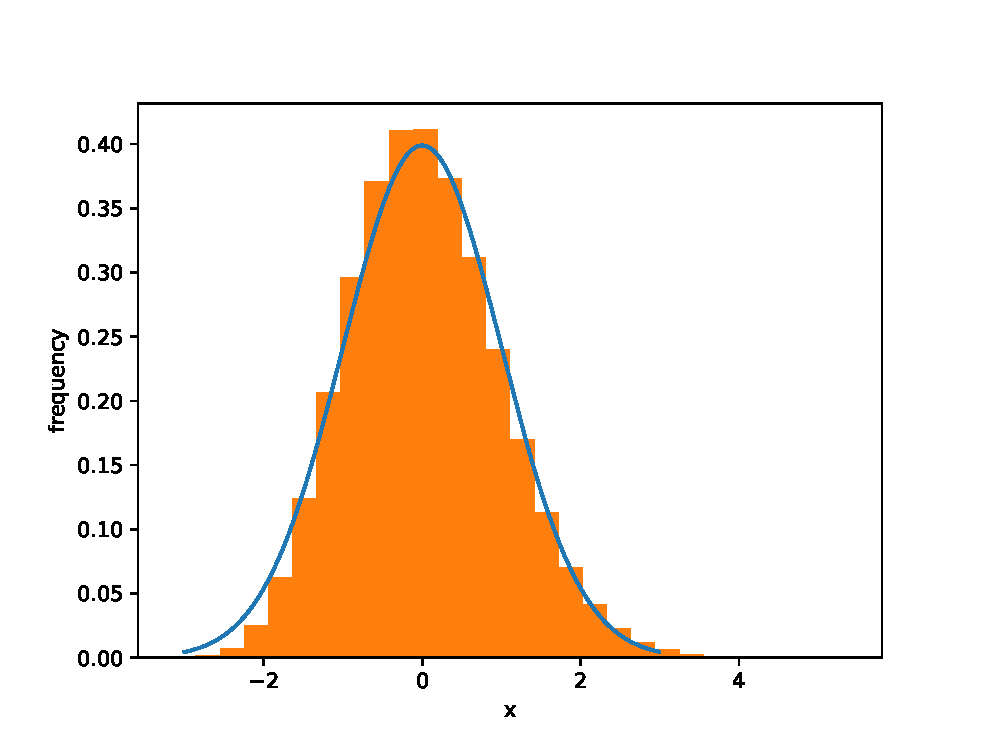
\includegraphics[width=0.33\textwidth]{poi_5_6.eps}}
    \hfill
    \caption{泊松分布抽样结果(N=5)}
\end{figure}

\begin{figure}[htb]
    \centering
    \subfloat[$n=10^2$]{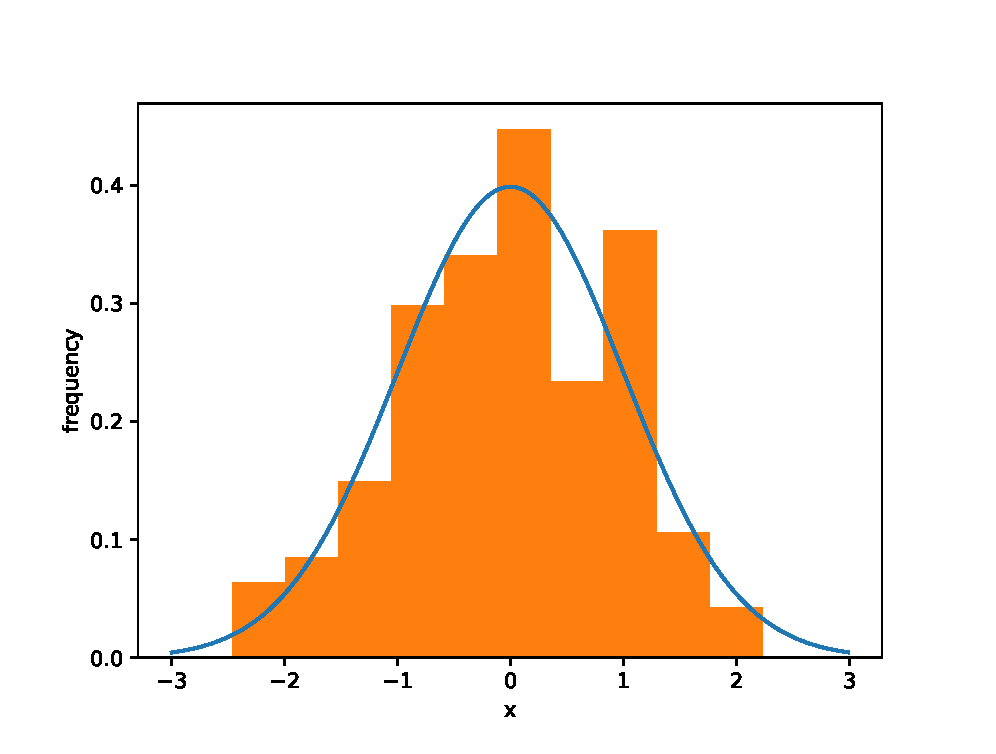
\includegraphics[width=0.33\textwidth]{poi_10_2.eps}}
    \hfill
    \subfloat[$n=10^4$]{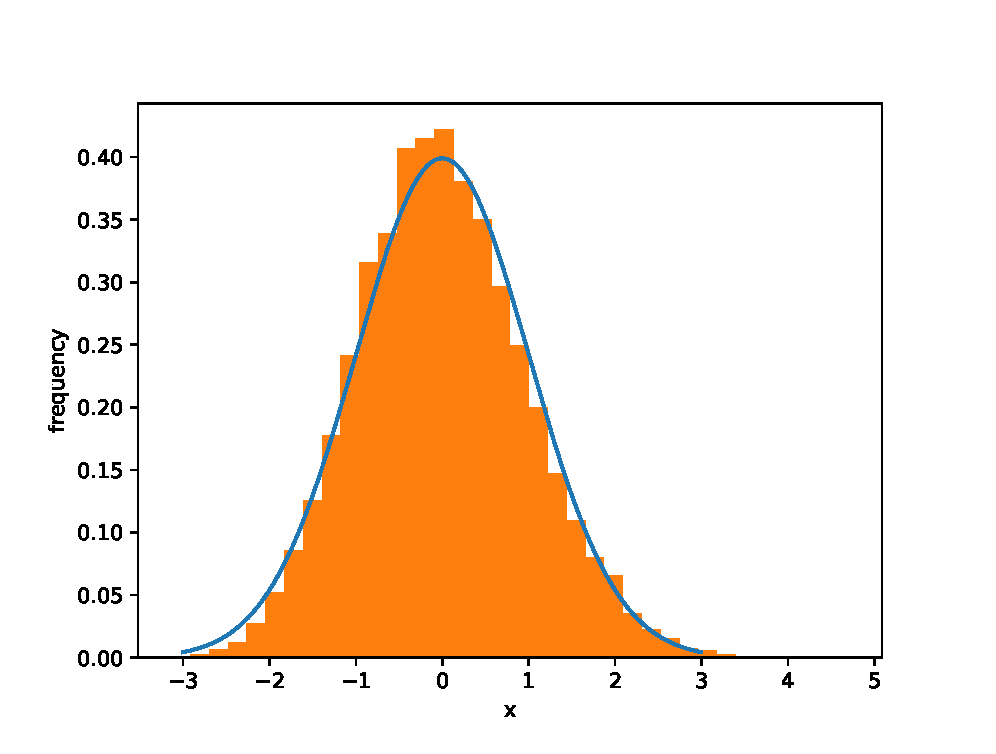
\includegraphics[width=0.33\textwidth]{poi_10_4.eps}}
    \hfill
    \subfloat[$n=10^6$]{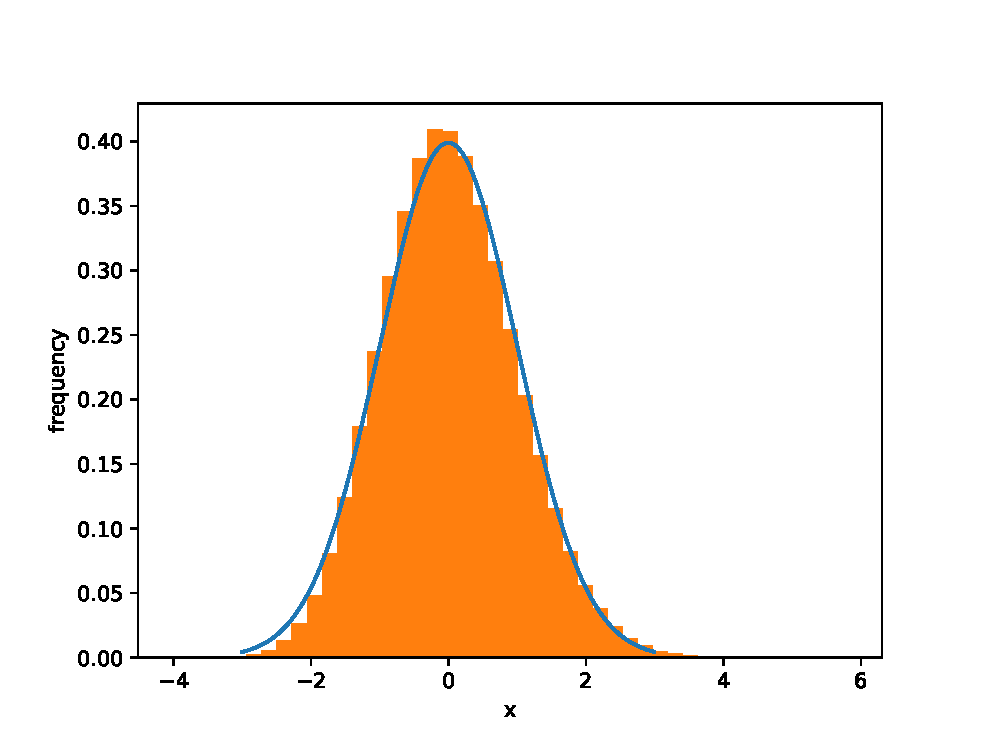
\includegraphics[width=0.33\textwidth]{poi_10_6.eps}}
    \hfill
    \caption{泊松分布抽样结果(N=10)}
\end{figure}

由于泊松分布是离散抽样,故选取区间只能比较宽才能等到理想的效果.
可见实际峰比理论峰要偏左,这是由于我们舍弃了$k$较大时的情形,
是一个“近似”的泊松分布. 

\subsection{指数分布抽样结果}

\begin{figure}[htb]
    \centering
    \subfloat[$n=10^2$]{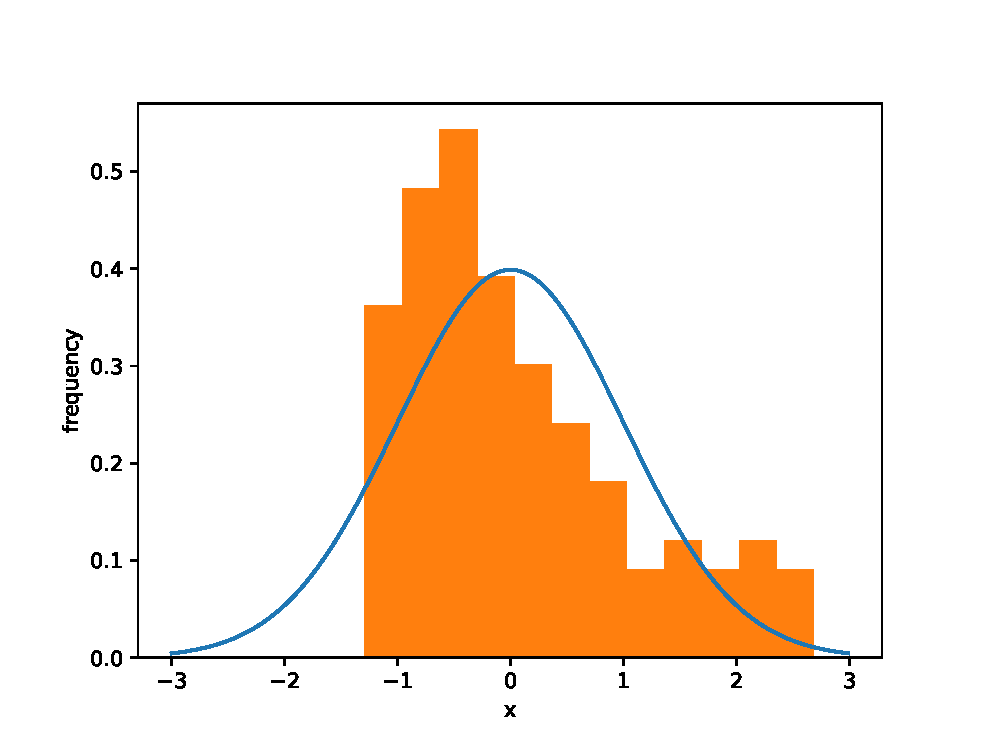
\includegraphics[width=0.33\textwidth]{expt_2_2.eps}}
    \hfill
    \subfloat[$n=10^4$]{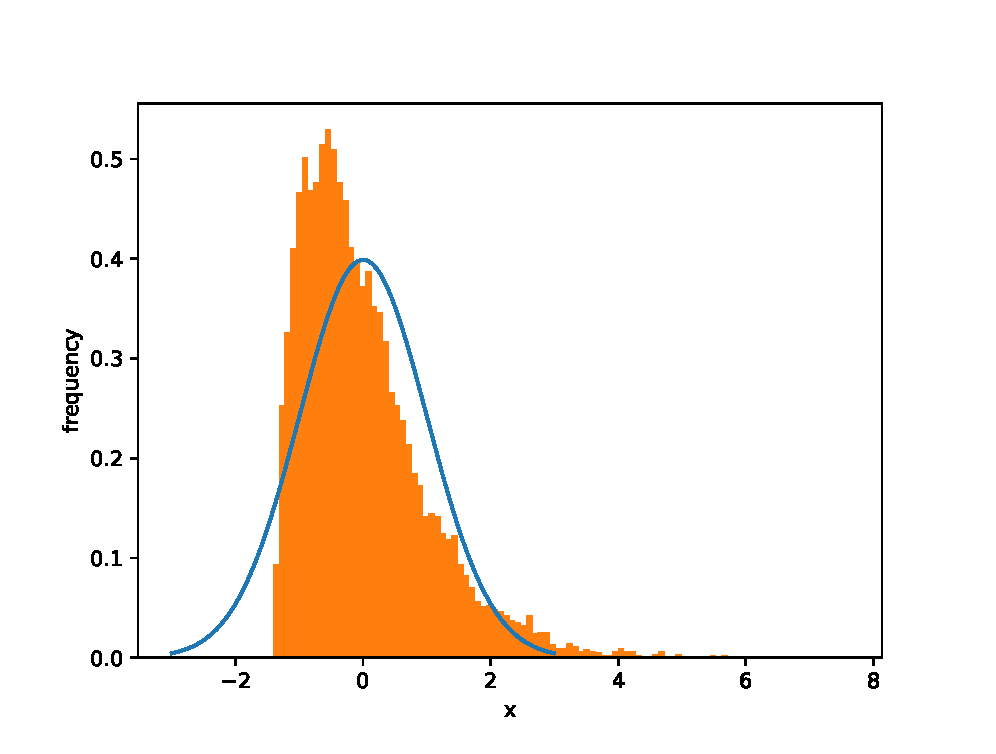
\includegraphics[width=0.33\textwidth]{expt_2_4.eps}}
    \hfill
    \subfloat[$n=10^6$]{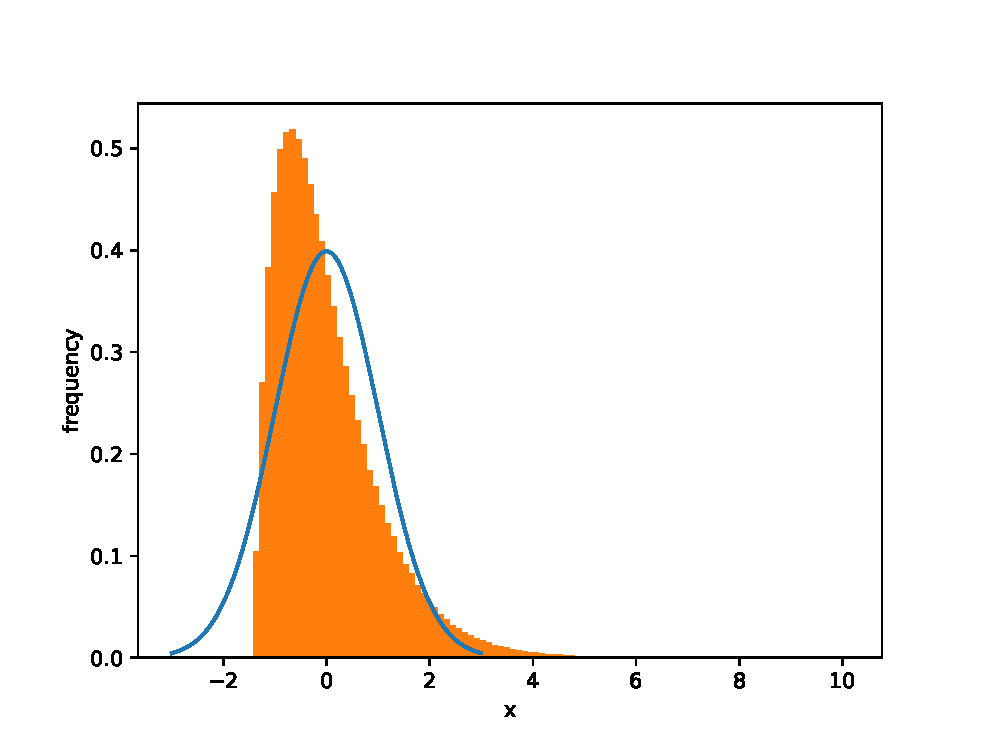
\includegraphics[width=0.33\textwidth]{expt_2_6.eps}}
    \hfill
    \caption{指数分布抽样结果(N=2)}
\end{figure}
\begin{figure}[htb]
    \centering
    \subfloat[$n=10^2$]{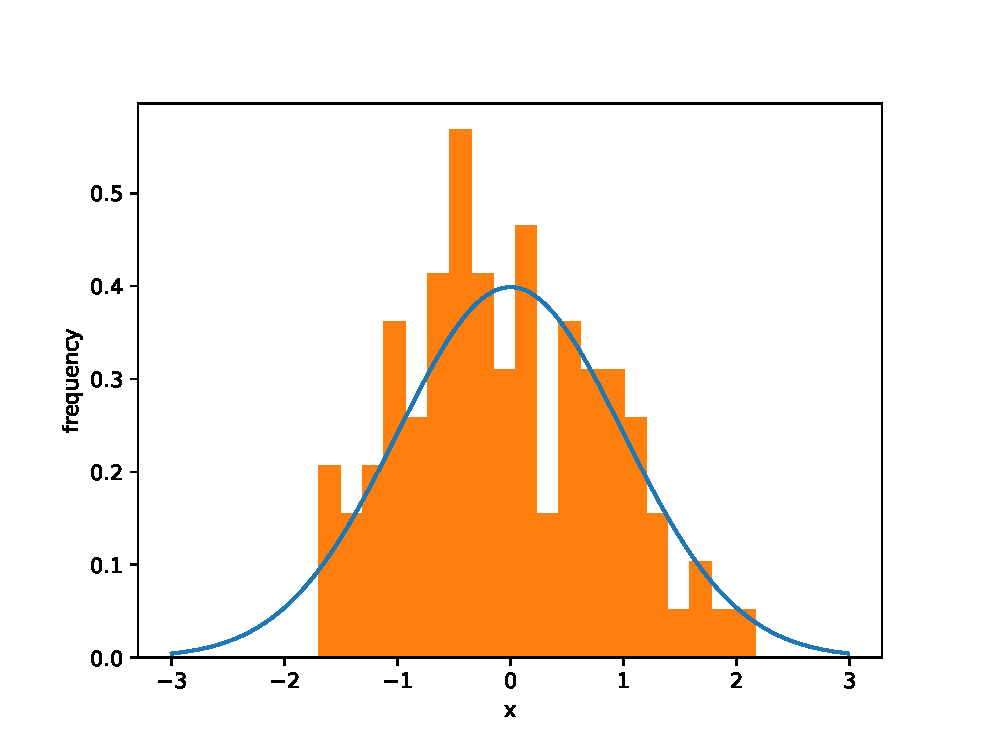
\includegraphics[width=0.33\textwidth]{expt_5_2.eps}}
    \hfill
    \subfloat[$n=10^4$]{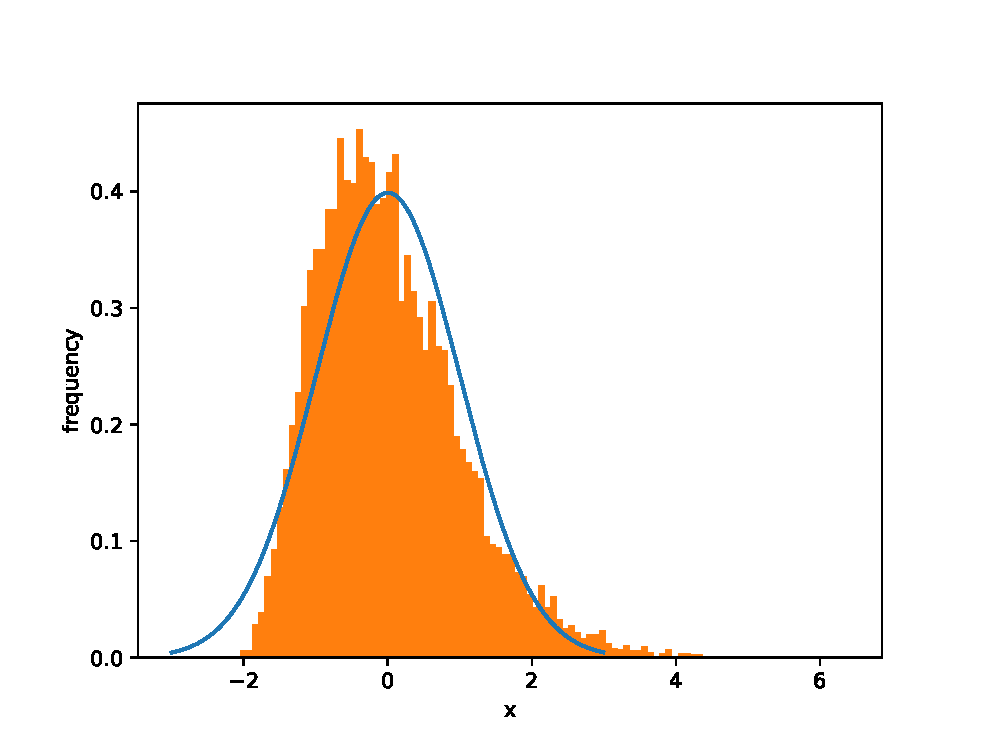
\includegraphics[width=0.33\textwidth]{expt_5_4.eps}}
    \hfill
    \subfloat[$n=10^6$]{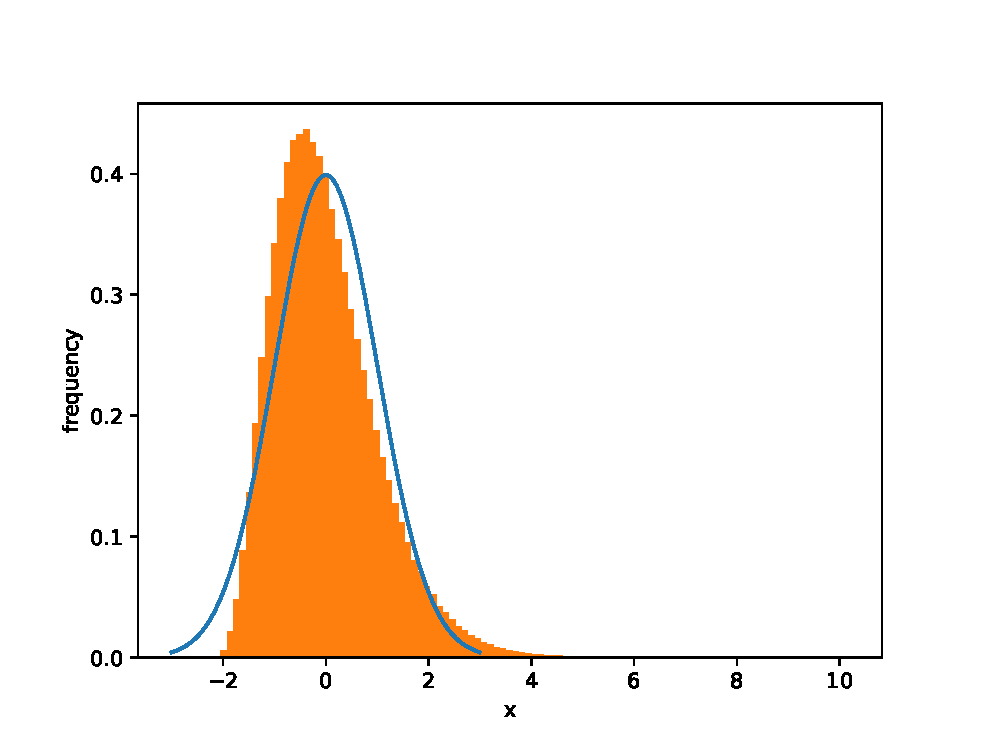
\includegraphics[width=0.33\textwidth]{expt_5_6.eps}}
    \hfill
    \caption{指数分布抽样结果(N=5)}
\end{figure}
\begin{figure}[htb]
    \centering
    \subfloat[$n=10^2$]{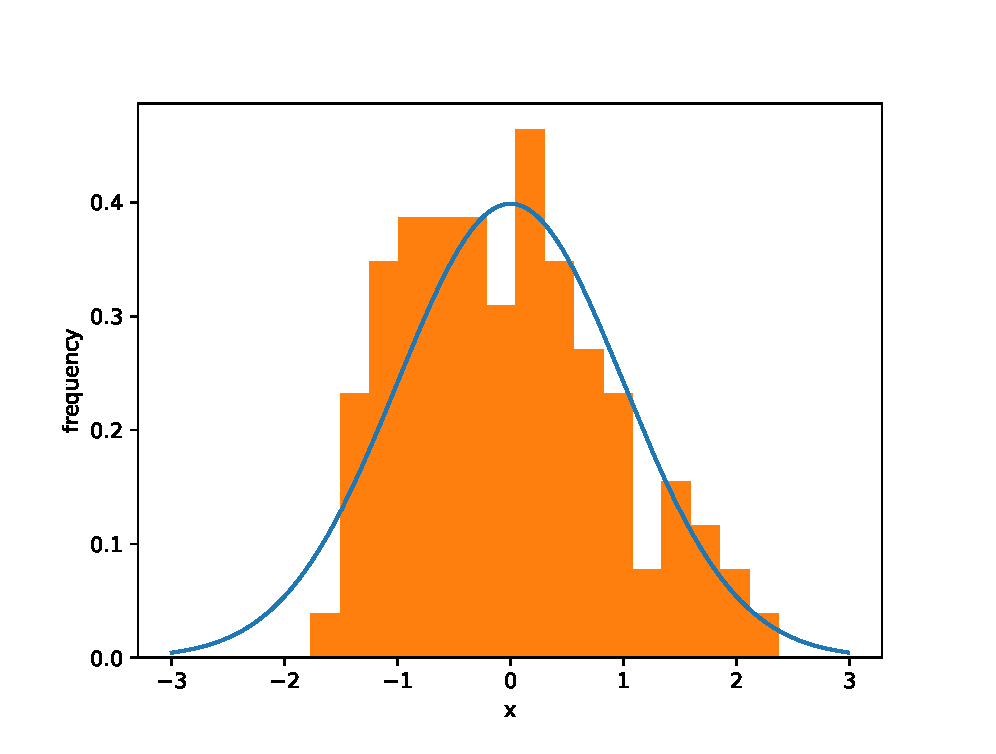
\includegraphics[width=0.33\textwidth]{expt_10_2.eps}}
    \hfill
    \subfloat[$n=10^4$]{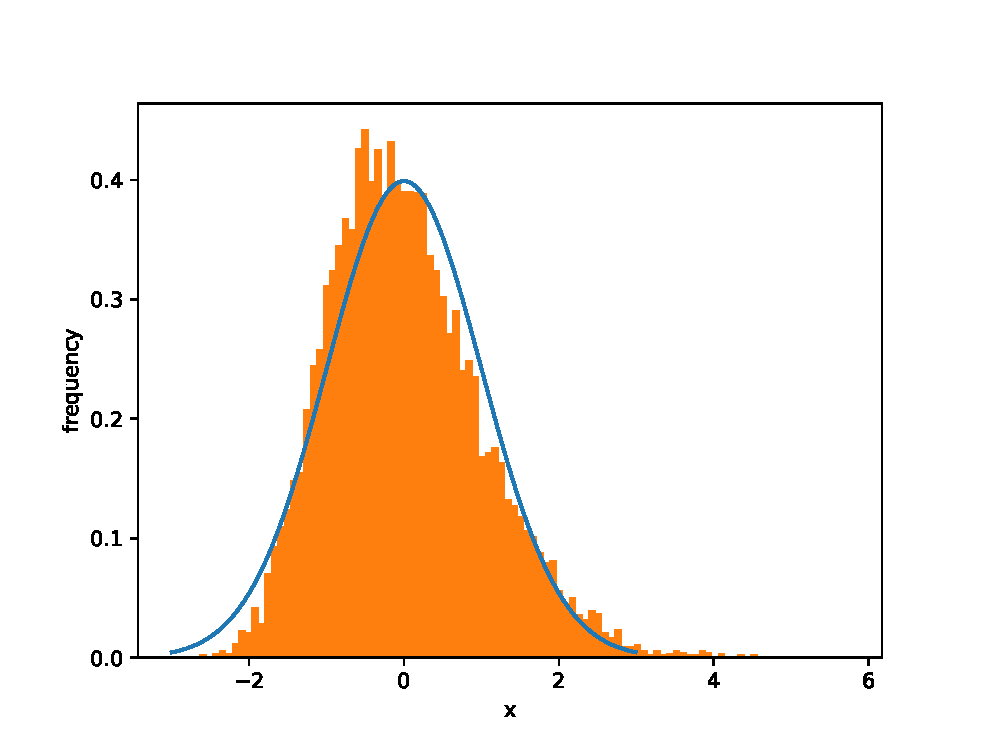
\includegraphics[width=0.33\textwidth]{expt_10_4.eps}}
    \hfill
    \subfloat[$n=10^6$]{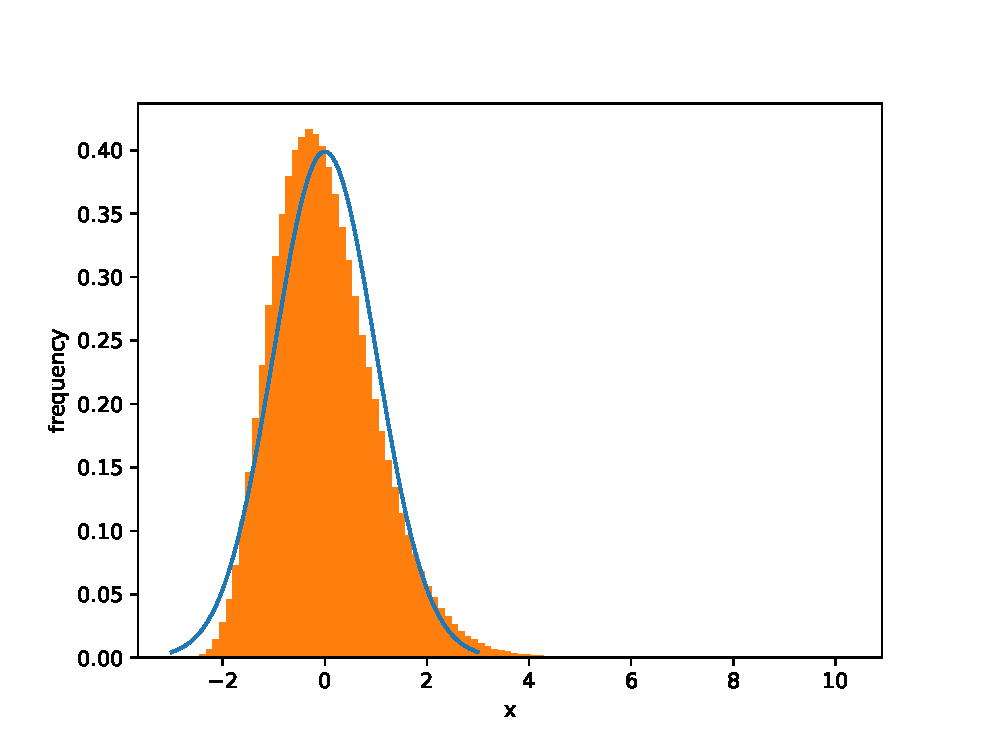
\includegraphics[width=0.33\textwidth]{expt_10_6.eps}}
    \hfill
    \caption{指数分布抽样结果(N=10)}
\end{figure}
\newpage

我们容易看出此时频率直方图也明显地趋近与正态曲线,但是峰偏左的现象比前者更为明显,
尤其是当$N$取2时,这也是我们取部分区间抽样所导致的,并不影响我们证明中心极限定理.

\subsection{自设离散分布抽样结果}

\begin{figure}[htb]
    \centering
    \subfloat[$n=10^2$]{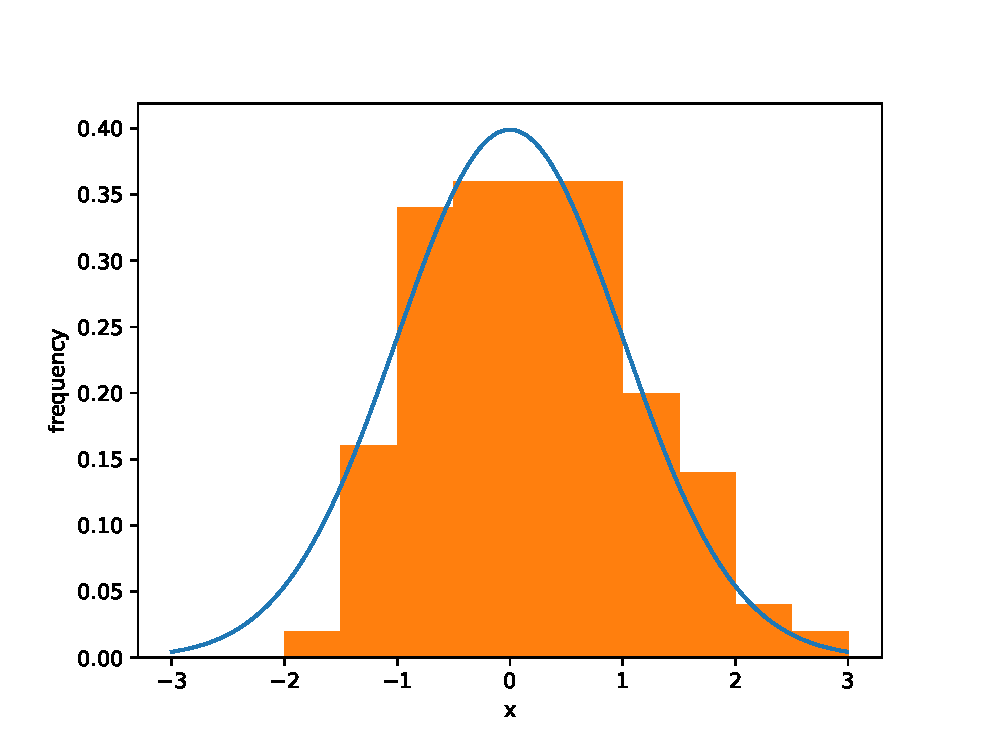
\includegraphics[width=0.33\textwidth]{mydsc_2_2.eps}}
    \hfill
    \subfloat[$n=10^4$]{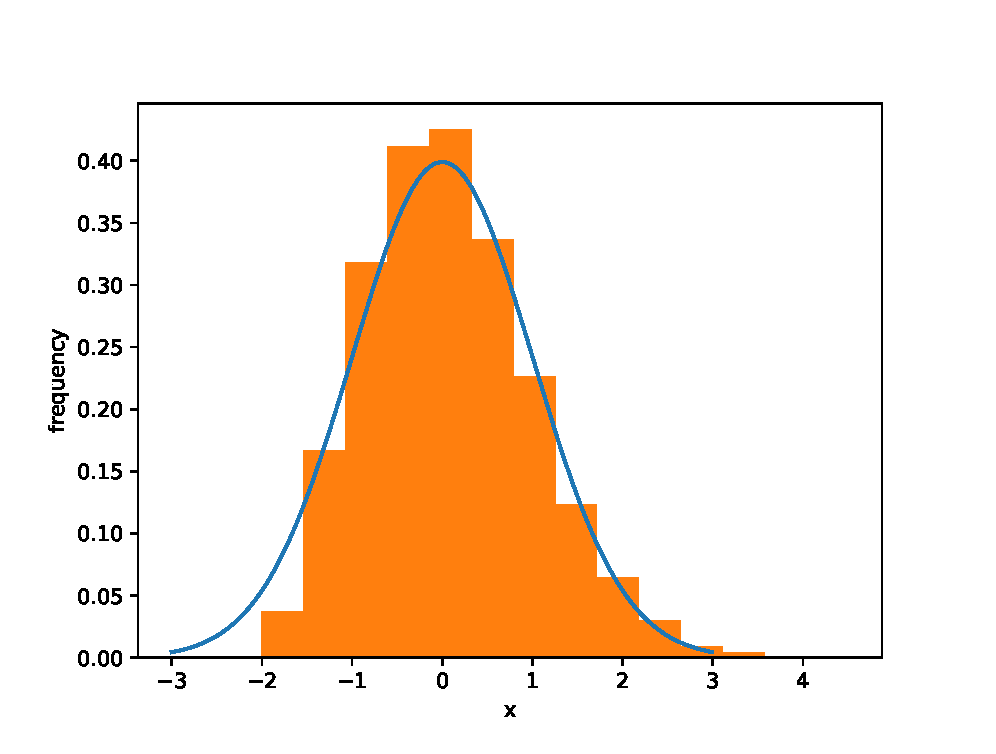
\includegraphics[width=0.33\textwidth]{mydsc_2_4.eps}}
    \hfill
    \subfloat[$n=10^6$]{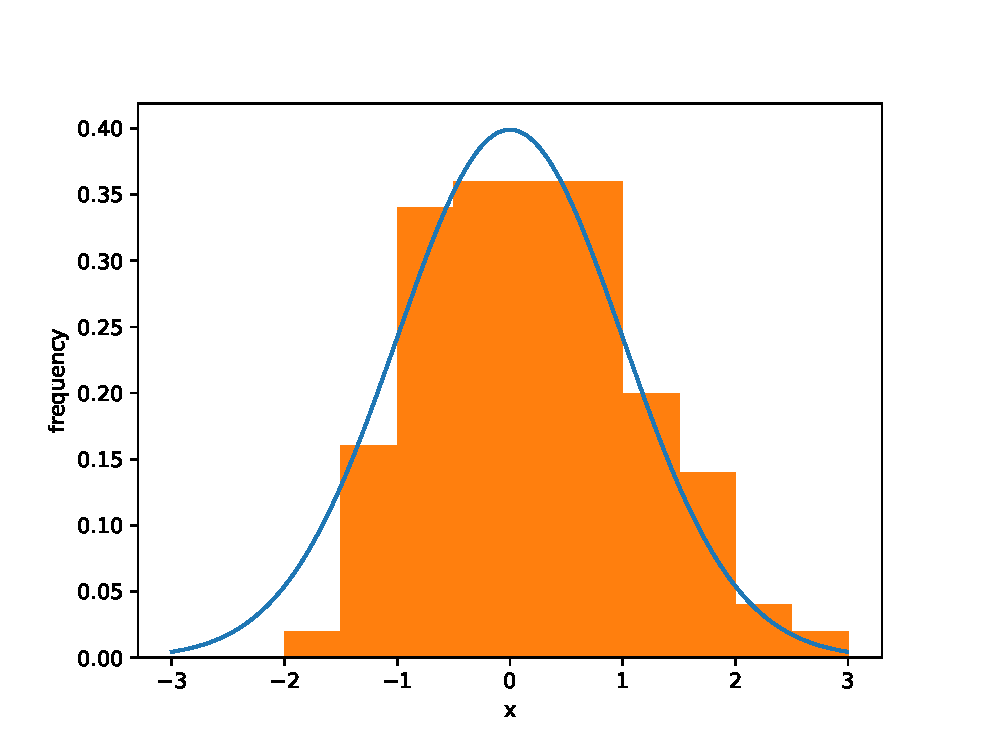
\includegraphics[width=0.33\textwidth]{mydsc_2_2.eps}}
    \hfill
    \caption{自设离散分布抽样结果(N=2)}
\end{figure}
\begin{figure}[htb]
    \centering
    \subfloat[$n=10^2$]{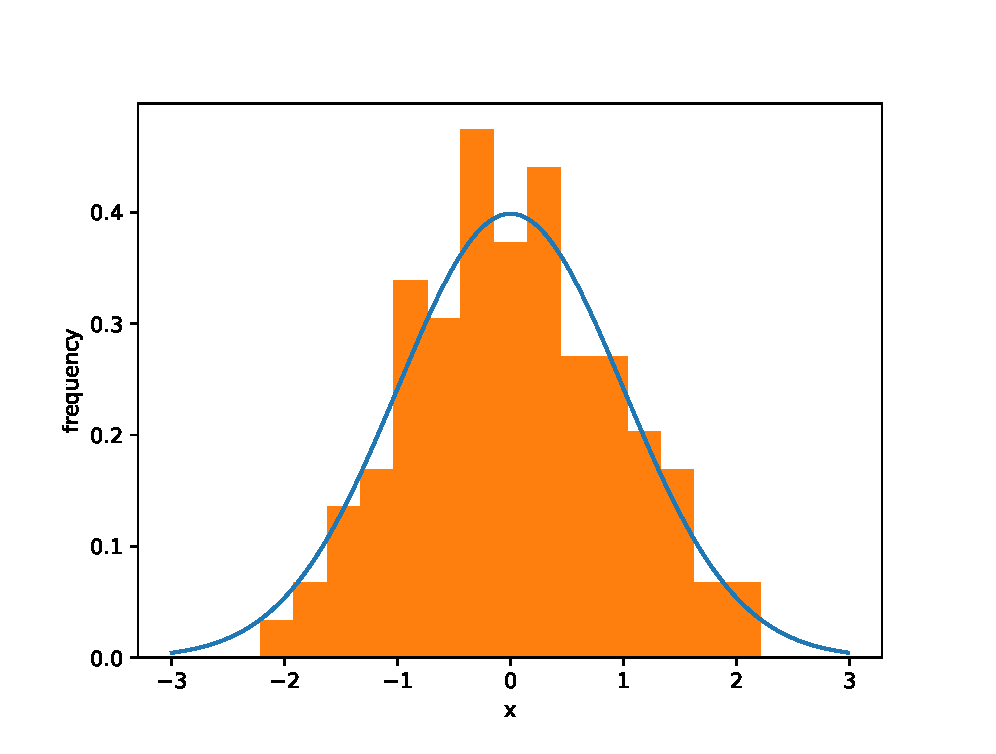
\includegraphics[width=0.33\textwidth]{mydsc_5_2.eps}}
    \hfill
    \subfloat[$n=10^4$]{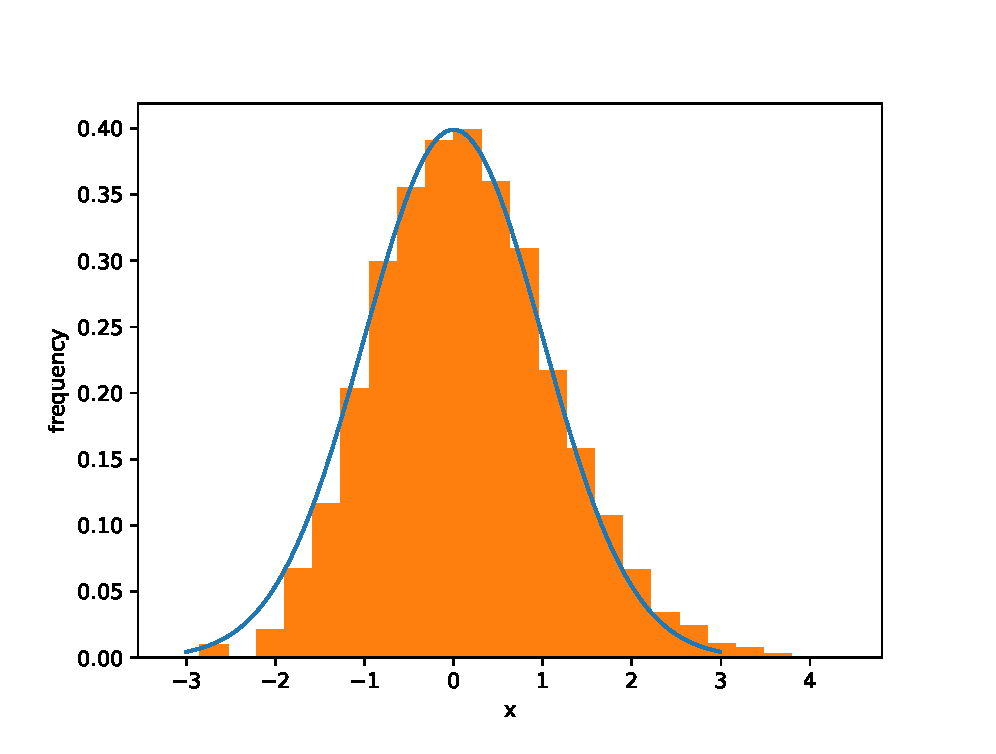
\includegraphics[width=0.33\textwidth]{mydsc_5_4.eps}}
    \hfill
    \subfloat[$n=10^6$]{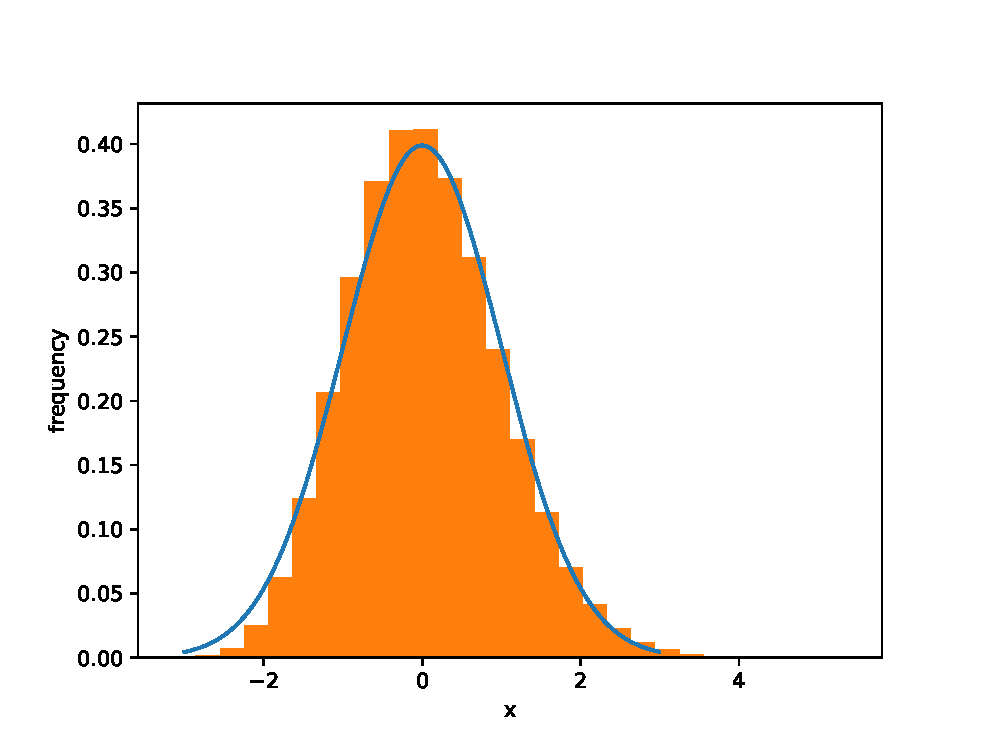
\includegraphics[width=0.33\textwidth]{mydsc_5_6.eps}}
    \hfill
    \caption{自设离散分布抽样结果(N=5)}
\end{figure}
\begin{figure}[htb]
    \centering
    \subfloat[$n=10^2$]{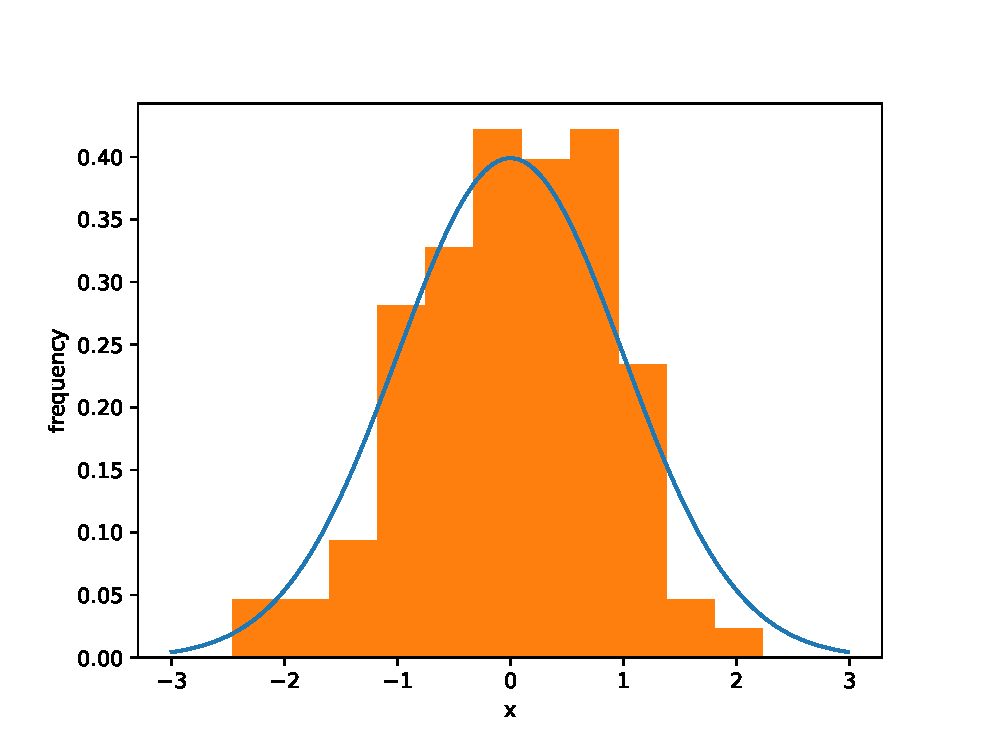
\includegraphics[width=0.33\textwidth]{mydsc_10_2.eps}}
    \hfill
    \subfloat[$n=10^4$]{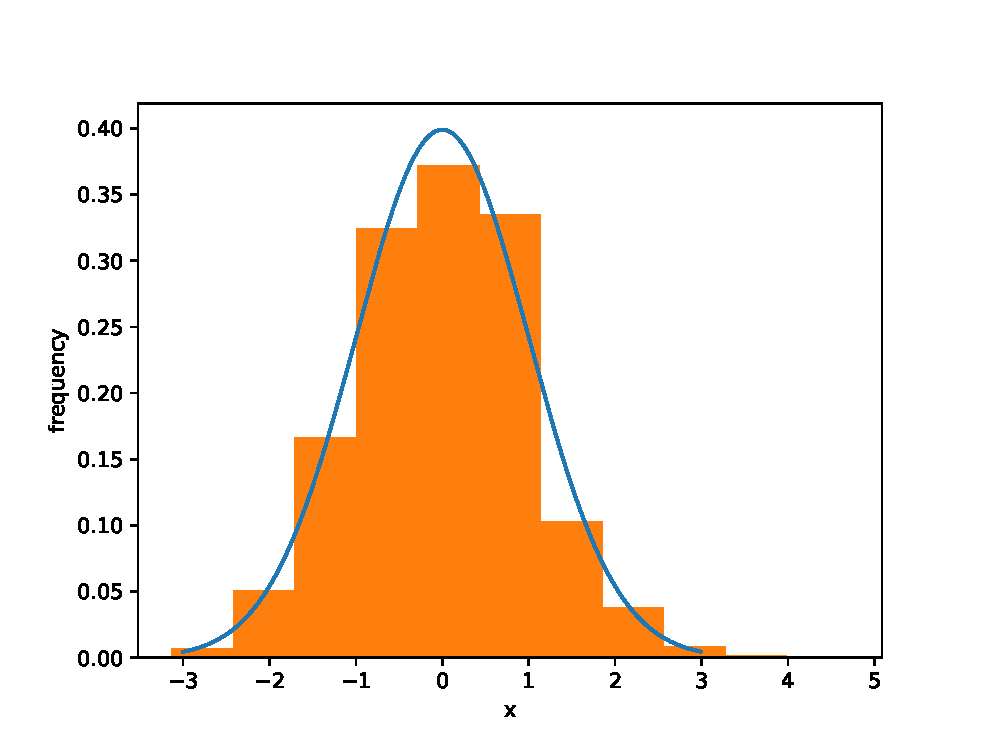
\includegraphics[width=0.33\textwidth]{mydsc_10_4.eps}}
    \hfill
    \subfloat[$n=10^6$]{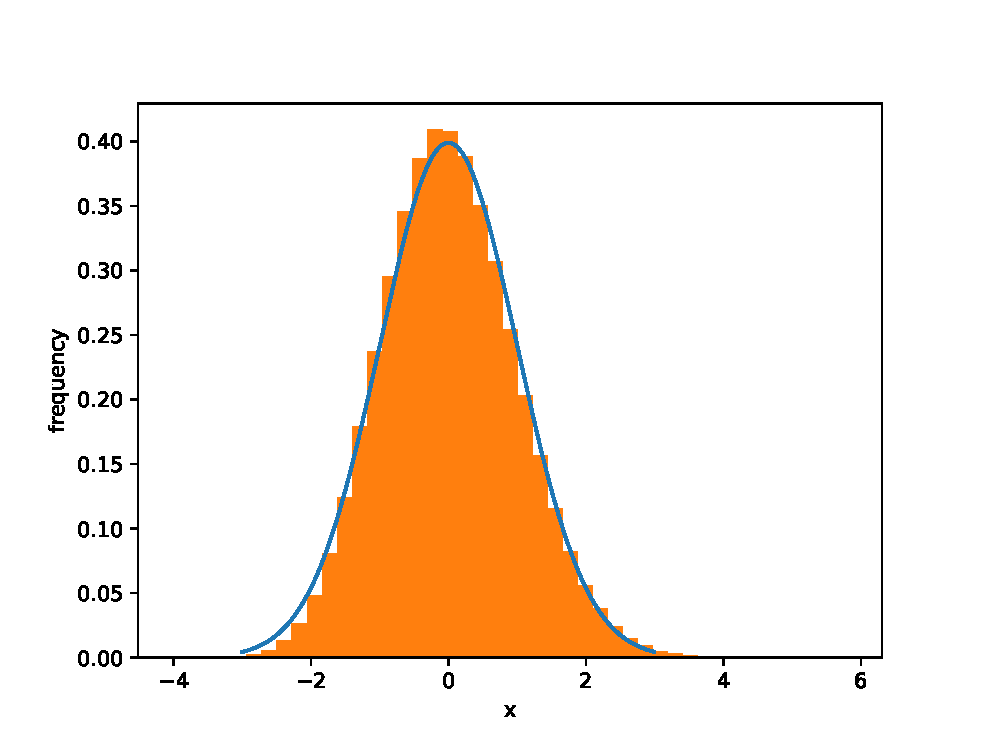
\includegraphics[width=0.33\textwidth]{mydsc_10_6.eps}}
    \hfill
    \caption{自设离散分布抽样结果(N=10)}
\end{figure}

由于所设函数较简单,$N=2$时频率直方图与正态曲线拟合不太好,但是当$N=5,10$时仍可明显看出
数据的正态分布趋势.

\subsection{自设连续分布抽样结果}

\begin{figure}[htb]
    \centering
    \subfloat[$n=10^2$]{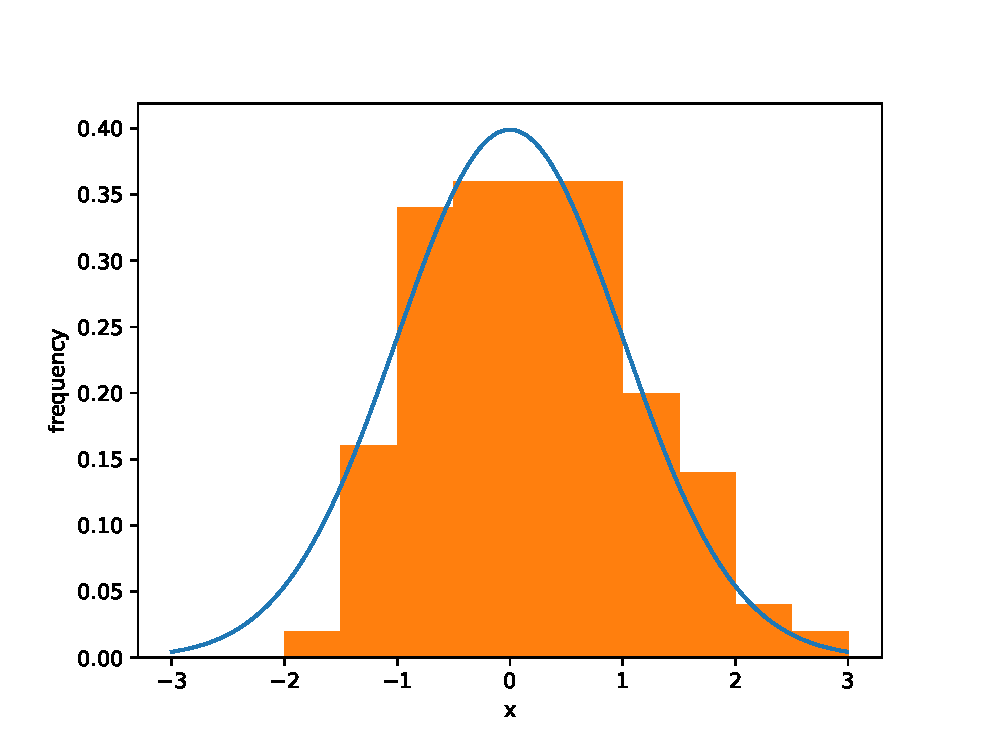
\includegraphics[width=0.33\textwidth]{myctn_2_2.eps}}
    \hfill
    \subfloat[$n=10^4$]{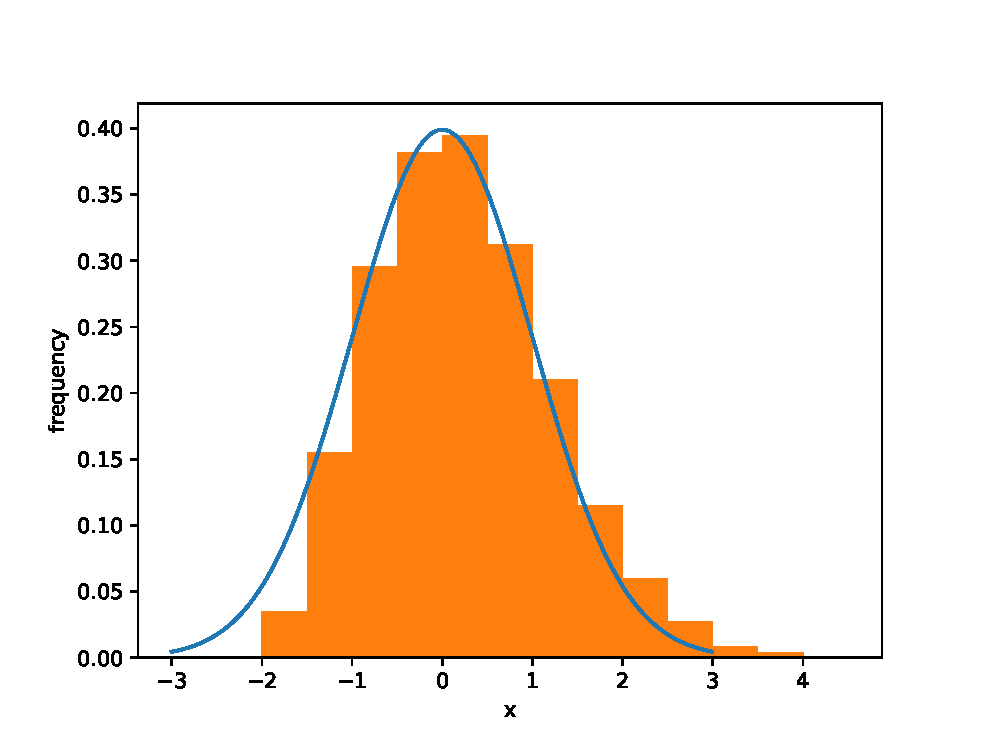
\includegraphics[width=0.33\textwidth]{myctn_2_4.eps}}
    \hfill
    \subfloat[$n=10^6$]{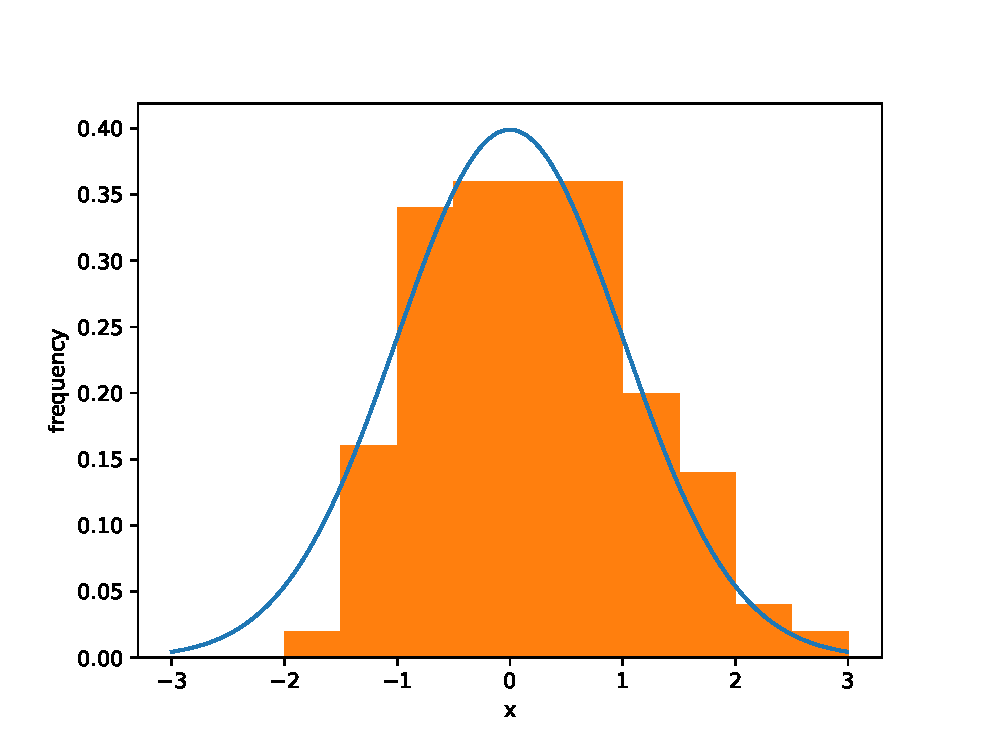
\includegraphics[width=0.33\textwidth]{myctn_2_2.eps}}
    \hfill
    \caption{自设连续分布抽样结果(N=2)}
\end{figure}
\begin{figure}[htb]
    \centering
    \subfloat[$n=10^2$]{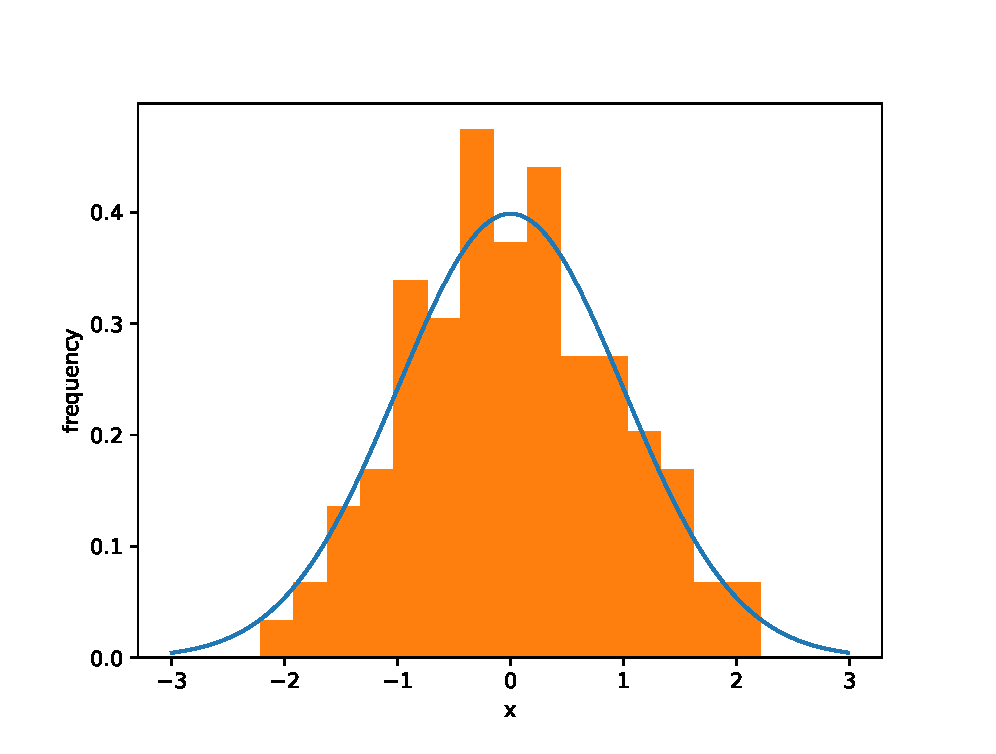
\includegraphics[width=0.33\textwidth]{myctn_5_2.eps}}
    \hfill
    \subfloat[$n=10^4$]{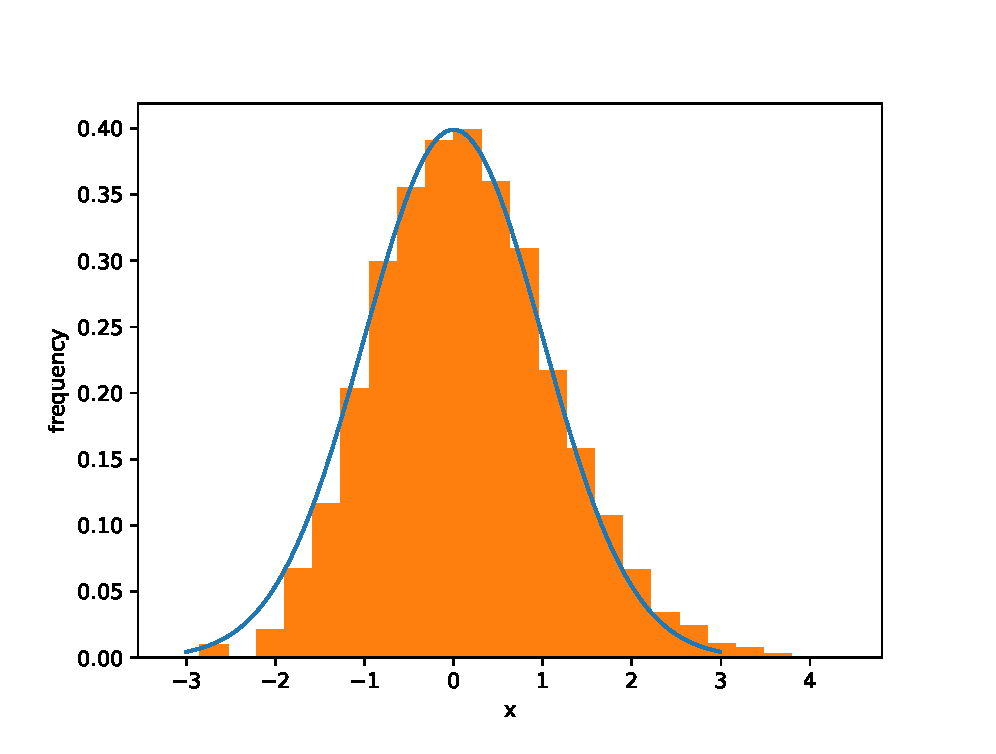
\includegraphics[width=0.33\textwidth]{myctn_5_4.eps}}
    \hfill
    \subfloat[$n=10^6$]{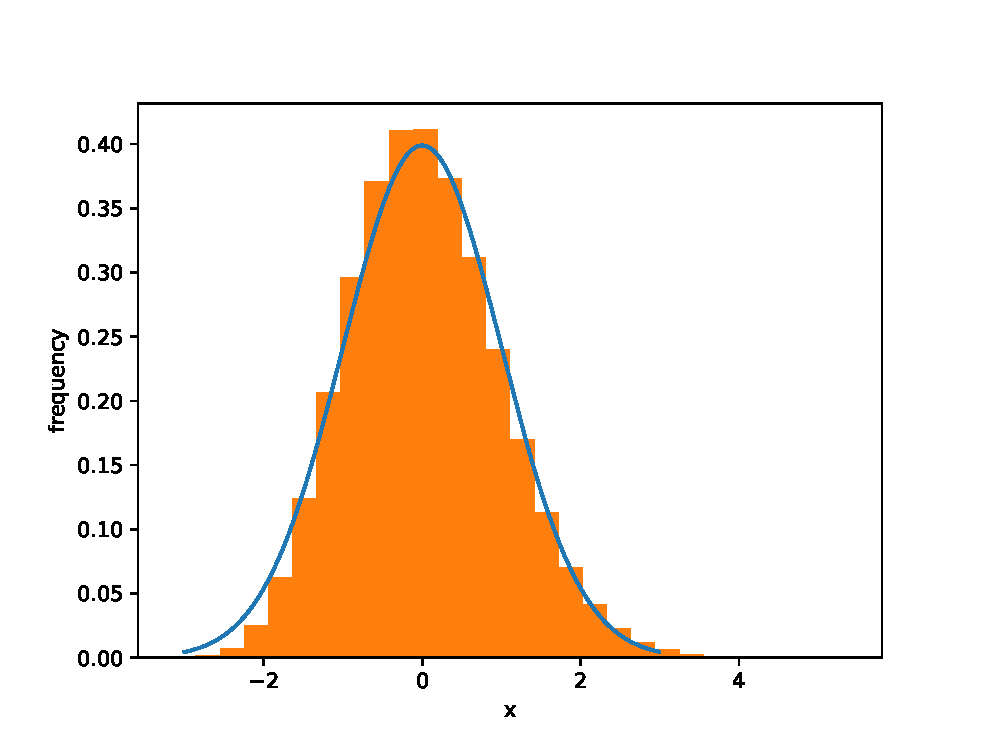
\includegraphics[width=0.33\textwidth]{myctn_5_6.eps}}
    \hfill
    \caption{自设连续分布抽样结果(N=5)}
\end{figure}
\begin{figure}[htb]
    \centering
    \subfloat[$n=10^2$]{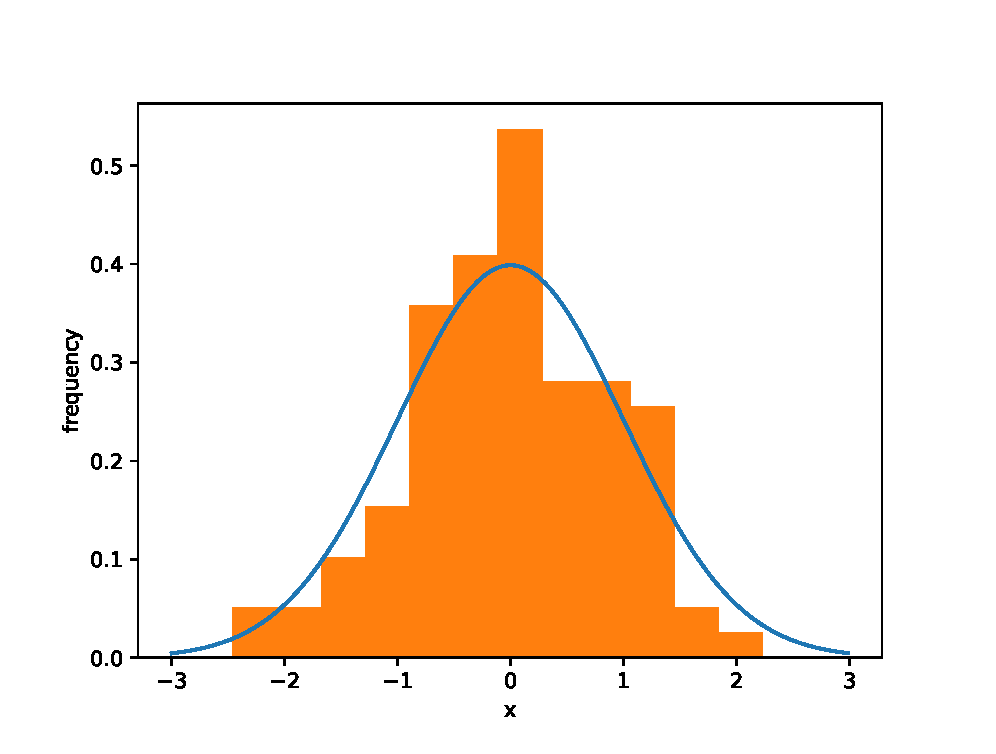
\includegraphics[width=0.33\textwidth]{myctn_10_2.eps}}
    \hfill
    \subfloat[$n=10^4$]{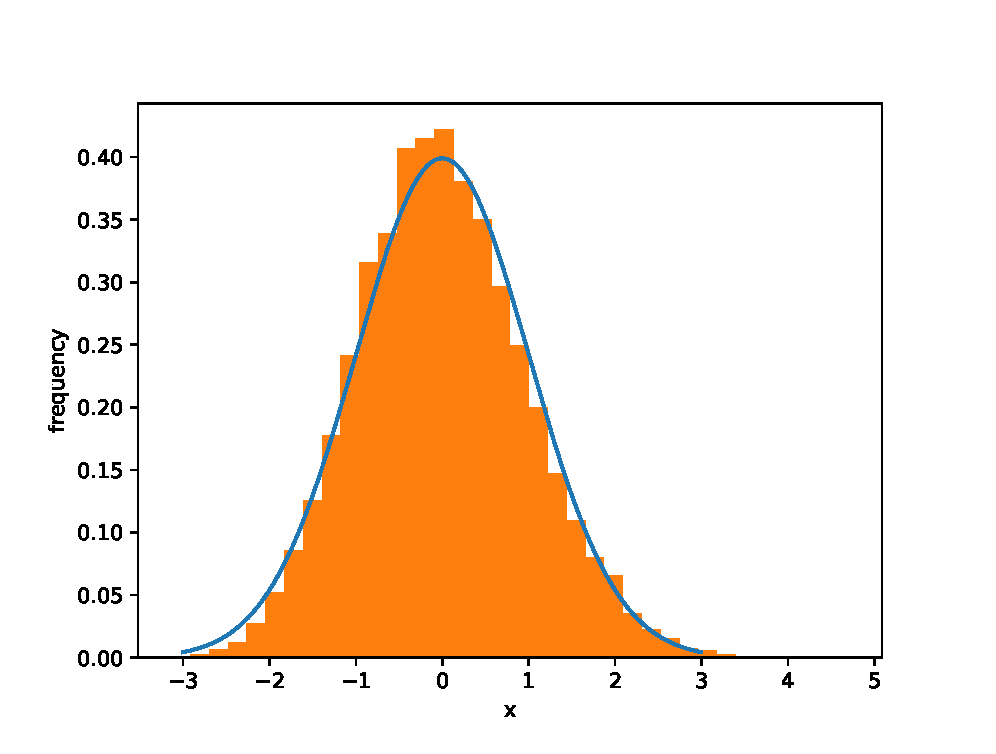
\includegraphics[width=0.33\textwidth]{myctn_10_4.eps}}
    \hfill
    \subfloat[$n=10^6$]{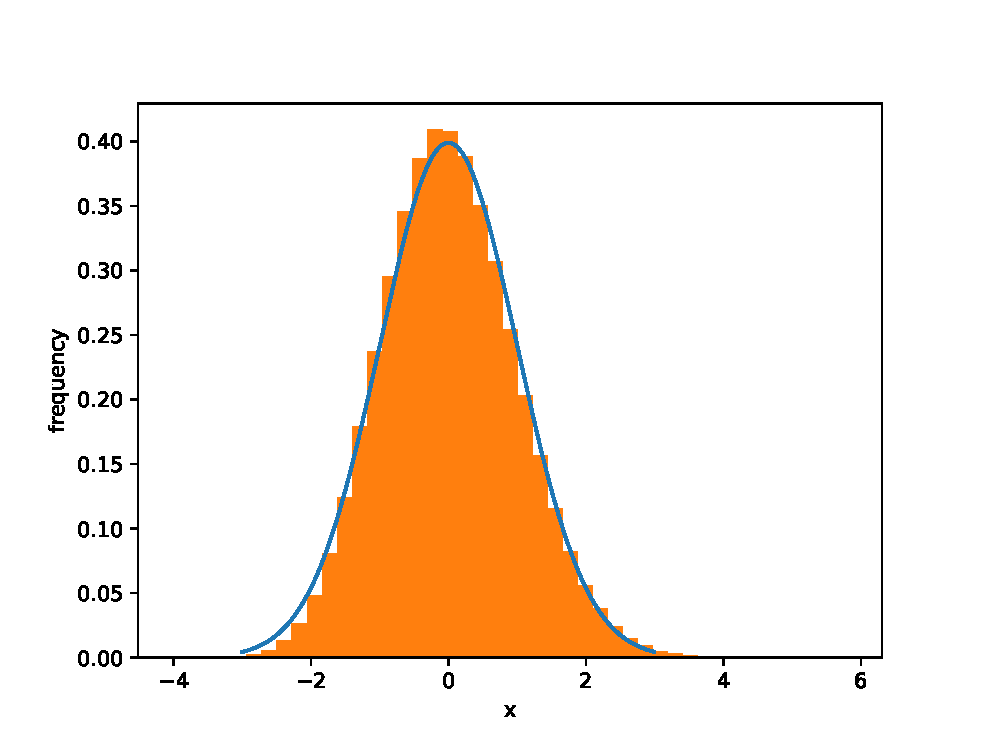
\includegraphics[width=0.33\textwidth]{myctn_10_6.eps}}
    \hfill
    \caption{自设连续分布抽样结果(N=10)}
\end{figure}

与上一节相似,当$N$更大时抽样结果与正态分布的吻合度更高.
\newpage
\section{结论}

综上,我们验证了泊松分布、指数分布以及自设的离散和连续分布满足中心极限定理.

\section{源程序}
将FORTRAN90源代码展示如下:

\begin{framed}
\begin{lstlisting}[language=Fortran]
MODULE DscSample !离散抽样模块
IMPLICIT NONE
CONTAINS

SUBROUTINE Poi(N, num, filename) !泊松分布的抽样以及统计量计算
    INTEGER(KIND=4) :: k, N, i, j, l, num
    REAL(KIND=8), DIMENSION(num * N) :: dat
    REAL(KIND=8), DIMENSION(num) :: g, xbar
    REAL(KIND=8), DIMENSION(num, N) :: x
    REAL(KIND=8), DIMENSION(0:8) :: sumprob
    REAL(KIND=8) :: maximum
    CHARACTER(LEN=*) :: filename
    CALL Schrage(num * N, 98412123, 'rand.dat') !共需要(n*N)个随机数
    OPEN (1, file='rand.dat')
    READ (1, *) dat
    CLOSE (1)
    sumprob(0) = f(0)
    DO i = 1, 8
        sumprob(i) = sumprob(i - 1) + f(i) !求分段节点
    END DO
    maximum = sumprob(8) 
    sumprob = sumprob / maximum !重新归一化
    DO i = 1, num
        DO j = 1, N
            DO l = 0, 8
                IF(dat((i * N - j + 1)) < sumprob(l)) THEN
                    x(i, j) = l !在指定概率区间内则取相应值
                    EXIT
                END IF
            END DO
        END DO
    END DO
    xbar = SUM(x, DIM=2) / N !通过数组运算求出每次循环中的平均值   
    g = SQRT(real(N) / 2) * (xbar - 2) !构造统计量
    OPEN (1, file=trim(filename))
    WRITE (1, *) g
    CLOSE (1)
    CONTAINS
        FUNCTION f(t) !Poisson分布密度函数表达式
            REAL(KIND=8) :: f
            INTEGER(KIND=4) :: t, y, m
            y = 1 !给阶乘值赋初值1
            IF(t .NE. 0) THEN
                DO m = 1, t
                    y = y * m !求阶乘
                END DO
            END IF
            f = (2**t * EXP(-2.0)) / y
        END FUNCTION f  
END SUBROUTINE Poi

SUBROUTINE Mydsc(N, num, filename) !自设离散分布的抽样与统计量计算
    INTEGER(KIND=4) :: k, N, i, j, l, num
    REAL(KIND=8), DIMENSION(num * N) :: dat
    REAL(KIND=8), DIMENSION(num) :: g, xbar
    REAL(KIND=8), DIMENSION(num, N) :: x
    REAL(KIND=8), DIMENSION(1:5) :: sumprob
    CHARACTER(LEN=*) :: filename
    CALL Schrage(num * N, 98412123, 'rand.dat') !共需要(n*N)个随机数
    sumprob(1) = 1.0 / 5
    DO i = 2, 5
        sumprob(i) = sumprob(i - 1) + 1.0 / 5
    END DO
    DO i = 1, num
        DO j = 1, N
            DO l = 1, 5
                IF(dat((i * N - j + 1)) < sumprob(l)) THEN
                    x(i, j) = l !在指定概率区间内则取相应值
                    EXIT
                END IF
            END DO
        END DO
    END DO
    xbar = SUM(x, DIM=2) / N !通过数组运算求出每次循环中的平均值   
    g = (xbar - 3) * SQRT(real(N) / 2) !计算统计量
    OPEN (1, file=filename)
    READ (1, *) g
    CLOSE (1)
END SUBROUTINE Mydsc
END MODULE DscSample

MODULE Sample !连续抽样模块
IMPLICIT NONE
    
CONTAINS
SUBROUTINE Expt(N, num, filename) !指数分布抽样与统计量计算
    INTEGER(KIND=4) :: N, num, i, j
    CHARACTER(LEN=*) :: filename
    REAL(KIND=8), DIMENSION(num * N) :: dat
    REAL(KIND=8), DIMENSION(num) :: g, xbar
    REAL(KIND=8), DIMENSION(num, N) :: x
    CALL Schrage(num * N, 7521233, 'rand.dat')
    OPEN (1, file='rand.dat')
    READ (1, *) dat
    CLOSE (1)
    DO i = 1, num
        DO j = 1, N
            x(i, j) = f(dat(i * N - j + 1)) !对0到1间均匀随机数直接抽样
        END DO
    END DO  
    xbar = SUM(x, DIM=2) / N !通过数组运算求出每次循环中的平均值   
    g = SQRT(real(N)) * (xbar - 1)
    OPEN (1, file=filename)
    WRITE (1, *) g
    CLOSE (1)
    CONTAINS
        FUNCTION f(t) !指数分布抽样函数
            REAL(KIND=8) :: f, t
            f = - LOG(t) !对f进行积分得到x平均值
        END FUNCTION f  
END SUBROUTINE Expt

SUBROUTINE Myctn(N, num, filename) !自设连续分布抽样与统计量计算
    INTEGER(KIND=4) :: N, num, i, j
    CHARACTER(LEN=*) :: filename
    REAL(KIND=8), DIMENSION(num * N) :: dat
    REAL(KIND=8), DIMENSION(num) :: g, xbar
    REAL(KIND=8), DIMENSION(num, N) :: x
    CALL Schrage(num * N, 64563218, 'rand.dat')
    OPEN (1, file='rand.dat')
    READ (1, *) dat
    CLOSE (1)
    DO i = 1, num
        DO j = 1, N
            x(i, j) = f(dat(i * N - j + 1)) !对0到1间均匀随机数直接抽样
        END DO
    END DO  
    xbar = SUM(x, DIM=2) / N !通过数组运算求出每次循环中的平均值   
    g = 2 * SQRT(real(N) / 5) * (3 * xbar - 1)
    OPEN (1, file=filename)
    WRITE (1, *) g
    CLOSE (1)
    CONTAINS
        FUNCTION f(t) !定义抽样函数
            REAL(KIND=8) :: f, t
            f = SQRT(2 * t)
        END FUNCTION f
END SUBROUTINE Myctn
END MODULE Sample

SUBROUTINE Schrage(num, z0, filename) !Schrage随机数生成器子程序
    IMPLICIT NONE
    INTEGER(KIND=4) :: N = 1, num
    INTEGER :: m = 2147483647, a = 16807, q = 127773, r = 2836, In(num), z0
    REAL(KIND=8) :: z(num)
    CHARACTER(LEN=8) :: filename
    In(1) = z0 !将传入值z0作为种子
    z(1) = REAL(In(1))/m
    DO N = 1, num - 1
        In(N + 1) = a*MOD(In(N), q) - r*INT(In(N)/q)
        IF (In(N + 1) < 0) THEN !若值小于零,按Schrage方法加m
            In(N + 1) = In(N + 1) + m
        END IF
        z(N + 1) = REAL(In(N + 1))/m !得到第N+1个随机数
    END DO
    OPEN (1, file=trim(filename)) !每次运行子程序按照传入参数filename生成数据文件
    DO N = 1, num !将随机数按行存入文件
        WRITE (1, *) z(N)
    END DO
    CLOSE (1)
END SUBROUTINE Schrage

PROGRAM MAIN
    USE DscSample
    USE Sample
    IMPLICIT NONE
    INTEGER(KIND=4) :: i, j
    CHARACTER(LEN=1) :: chari 
    DO i = 2, 6, 2
        WRITE (chari, "(I1)") i !将整型数值转化为字符型便于写入文件名
        CALL Poi(2, 10**i, 'poi_2_' // chari // '.dat') 
        CALL Poi(5, 10**i, 'poi_5_' // chari // '.dat')
        CALL Poi(10, 10**i, 'poi_10_' // chari // '.dat')
        WRITE (chari, "(I1)") i
        CALL Expt(2, 10**i, 'expt_2_' // chari // '.dat') 
        CALL Expt(5, 10**i, 'expt_5_' // chari // '.dat')
        CALL Expt(10, 10**i, 'expt_10_' // chari // '.dat')
        WRITE (chari, "(I1)") i
        CALL Poi(2, 10**i, 'mydsc_2_' // chari // '.dat') 
        CALL Poi(5, 10**i, 'mydsc_5_' // chari // '.dat')
        CALL Poi(10, 10**i, 'mydsc_10_' // chari // '.dat')
        WRITE (chari, "(I1)") i
        CALL Poi(2, 10**i, 'myctn_2_' // chari // '.dat') 
        CALL Poi(5, 10**i, 'myctn_5_' // chari // '.dat')
        CALL Poi(10, 10**i, 'myctn_10_' // chari // '.dat')
    END DO
END PROGRAM MAIN

\end{lstlisting}
\end{framed}

以及使用多次的python脚本:
\begin{framed}
\begin{lstlisting}[language=python]
import numpy as np
import matplotlib.pyplot as plt
import math

plt.rcParams['savefig.dpi'] = 300
plt.rcParams['figure.dpi'] = 300

x = np.arange(-3, 3, 0.01)
y = np.exp(-pow(x, 2) / 2) / np.sqrt(2 * np.pi)
data = np.loadtxt('myctn_2_6.dat')
plt.xlabel('x')
plt.ylabel('frequency')
plt.plot(x, y)
plt.hist(data, bins=16, density=True)
plt.savefig('myctn_2_6.eps')
plt.show()
\end{lstlisting}
\end{framed}
\end{document}
